%% ===========================================================================
%%  Attention-Masked Token Composition — IEEE TCSVT (IEEEtran journal) version
%%  Converted from the ACM MM submission (../ACM-MM_edited).
%%
%%  Build:  pdflatex main -> bibtex main -> pdflatex main -> pdflatex main
%%          (or: latexmk -pdf main.tex)
%%
%%  Submission note: TCSVT initial submissions are usually sent as a
%%  DOUBLE-SPACED single-column manuscript.  Use
%%      \documentclass[journal,onecolumn,draftclsnofoot,11pt]{IEEEtran}
%%  for the review copy, and the [journal] line below for the final/preprint
%%  two-column look.  Both compile from these same source files.
%% ===========================================================================

\documentclass[journal]{IEEEtran}
% \documentclass[journal,onecolumn,draftclsnofoot,11pt]{IEEEtran}  % review copy

\usepackage{cite}                 % IEEE-style compressed numeric citations
\usepackage[T1]{fontenc}
\usepackage{graphicx}
\usepackage{amsmath,amssymb,amsfonts}
\usepackage{booktabs}
\usepackage[table]{xcolor}
\usepackage{colortbl}
\usepackage{multirow}
\usepackage{algorithm}
\usepackage{algpseudocode}
\usepackage{subcaption}
\usepackage{pgf}
\usepackage[normalem]{ulem}       % normalem: keep \emph italic, only \uline underlines
\usepackage{microtype}
\usepackage{url}
\usepackage[hidelinks]{hyperref}

% algorithm + IEEEtran: keep the caption above the body and avoid float warnings
\renewcommand{\algorithmicrequire}{\textbf{Input:}}
\renewcommand{\algorithmicensure}{\textbf{Output:}}

% ---------------------------------------------------------------------------
% Heat-map cell shading used in the main comparison table (carried over from
% the ACM version; requires pgf + colortbl + [table]xcolor).
%
% Marking convention: a cell equal to the column extreme is set in bold; the
% fourth argument is the second-best flag and underlines the cell.
% ---------------------------------------------------------------------------
\newcommand{\MinShade}{0}
\newcommand{\MaxShade}{85}

% Higher is better
\newcommand{\AutoCellUp}[4]{%
  \begingroup
  \pgfmathparse{round(max(\MinShade,min(\MaxShade,\MinShade + (\MaxShade-\MinShade)*(((#1-#2)/(#3-#2))^2))))}%
  \edef\ShadeValue{\pgfmathresult}%
  \edef\ColorSpec{cyan!\ShadeValue}%
  \pgfmathparse{(#1==#3 ? 1 : 0)}%
  \ifnum\pgfmathresult=1
    \expandafter\cellcolor\expandafter{\ColorSpec}\textbf{#1}%
  \else
    \ifnum#4=1
      \expandafter\cellcolor\expandafter{\ColorSpec}\uline{#1}%
    \else
      \expandafter\cellcolor\expandafter{\ColorSpec}#1%
    \fi
  \fi
  \endgroup
}

% Lower is better
\newcommand{\AutoCellDown}[4]{%
  \begingroup
  \pgfmathparse{round(max(\MinShade,min(\MaxShade,\MinShade + (\MaxShade-\MinShade)*(((#3-#1)/(#3-#2))^2))))}%
  \edef\ShadeValue{\pgfmathresult}%
  \edef\ColorSpec{cyan!\ShadeValue}%
  \pgfmathparse{(#1==#2 ? 1 : 0)}%
  \ifnum\pgfmathresult=1
    \expandafter\cellcolor\expandafter{\ColorSpec}\textbf{#1}%
  \else
    \ifnum#4=1
      \expandafter\cellcolor\expandafter{\ColorSpec}\uline{#1}%
    \else
      \expandafter\cellcolor\expandafter{\ColorSpec}#1%
    \fi
  \fi
  \endgroup
}

% ---------------------------------------------------------------------------
\begin{document}

\title{Attention-Masked Token Composition for Training-Free
       Image Editing with Visual Autoregressive Models}

%% ===========================================================================
%%  AUTHOR BLOCK — LEFT BLANK ON PURPOSE.
%%
%%  >>> TODO(user): fill in real names / IEEE membership / affiliations /
%%  >>> e-mails / funding acknowledgement / corresponding author before
%%  >>> submission.  Everything below is a placeholder skeleton.
%%
%%  For the ANONYMOUS review copy, keep the \author{} block as-is
%%  (Anonymous Authors) and comment out the \thanks lines.
%% ===========================================================================

\author{%
  Anonymous~Author,%
  ~\IEEEmembership{Student Member,~IEEE,}
  Anonymous~Author,%
  ~\IEEEmembership{Member,~IEEE,}
  and~Anonymous~Author,%
  ~\IEEEmembership{Senior Member,~IEEE}%
  \thanks{Manuscript received XX XX, 20XX; revised XX XX, 20XX. % TODO
          This work was supported in part by \textit{[funding agency, grant no.]}.} % TODO
  \thanks{The authors are with the \textit{[Department]}, \textit{[University]},
          \textit{[City, Country]} (e-mail: \textit{[e-mail]}).} % TODO
  \thanks{Corresponding author: \textit{[name]}.} % TODO
  \thanks{Color versions of one or more figures in this article are available
          online at https://doi.org/XX.XXXX/TCSVT.20XX.XXXXXXX.} % TODO
  \thanks{Digital Object Identifier XX.XXXX/TCSVT.20XX.XXXXXXX}% TODO
}


% Running heads.  Replace the volume/number/date once the paper is accepted.
\markboth{IEEE Transactions on Circuits and Systems for Video Technology,~Vol.~XX, No.~XX, XXXX~20XX}%
{Author \MakeLowercase{\textit{et al.}}: Attention-Masked Token Composition for Training-Free Image Editing}

\maketitle

%% ===========================================================================
%%  Abstract + index terms (IEEE format).
%%  The ACM CCS concept block (\begin{CCSXML} ... \ccsdesc) has been removed:
%%  IEEE journals do not use CCS; keywords become \begin{IEEEkeywords}.
%%
%%  NOTE: this is still the ACM-submission abstract.  See
%%  docs/reports/TCSVT_migration_notes.md §2 for the recommended rewrite that
%%  matches the TCSVT positioning (systems/analysis framing, controllable
%%  preservation--edit trade-off, new evidence).
%% ===========================================================================

\begin{abstract}
Text-guided image editing aims to modify real images according to natural language instructions while preserving non-target visual content. Existing diffusion- and rectified flow-based methods face a fundamental trade-off between editing effectiveness and source fidelity, stemming from inversion errors inherent to continuous latent trajectories and cross-modal feature entanglement that causes unintended global changes. We present a \textbf{training-free text-guided image editing framework based on Visual Autoregressive Modeling (VAR)}, which sidesteps both challenges by operating on discrete, scale-wise token generation rather than continuous noise removal. Since no trajectory exists to invert, tokens can be selectively replaced at the sampling stage without altering the global generation process. Our method leverages cross-modal attention maps between text and visual tokens to automatically derive high-attention focus masks and low-attention preserve masks at each generation scale, eliminating the need for external segmentation tools or per-category hyperparameter tuning. Binarizing those maps is the step that governs the preservation--edit trade-off, and we show that rank-based and mean-relative thresholds both fail for the same structural reason; we instead threshold an absolute energy level on the normalized attention map with an instance-adaptive correction, whose parameters are calibrated so that the realized threshold distribution is centred on a chosen operating point rather than tuned by inspection. For real image editing, the source image is encoded into discrete per-scale bitwise tokens via BSQ-VAE, enabling direct token-level background substitution that faithfully preserves source content without inversion or continuous feature injection. Beyond the method, we systematically isolate which components govern the trade-off: the base threshold traces a smooth monotone frontier and is the single control worth exposing, the instance-adaptive correction is a small refinement on top of it rather than a second lever, the target-stream pass contributes structurally rather than parametrically, and one apparent hyperparameter provably cannot affect the output. On PIE-Bench our method attains the best SSIM and the best CLIP whole-image similarity among diffusion-, flow- and autoregressive-based training-free baselines, is second on LPIPS and on edited-region CLIP, and remains in the leading group on human-preference scores while using a 2B-parameter backbone --- six times smaller than the flow-based baselines --- in an inversion-free pipeline that runs in about 2.5 seconds per image.
\end{abstract}

\begin{IEEEkeywords}
Image editing, text-guided image manipulation, visual autoregressive modeling, training-free editing, inversion-free editing, cross-modal attention, discrete token representation.
\end{IEEEkeywords}


\IEEEpeerreviewmaketitle

% --- Teaser (was \begin{teaserfigure} in acmart; IEEE has no equivalent, so it
% --- becomes an ordinary full-width float).
\begin{figure*}[!t]
  \centering
  \includegraphics[width=\textwidth]{teaser/imageEditing.png}
  \caption{Diverse editing results of our training-free, inversion-free framework on a 2B-parameter VAR model. Each pair shows source and edited images side by side or top and bottom, spanning object replacement, addition and attribute modification. Our method constructs attention-driven spatial masks and performs discrete token-level composition, achieving precise edits with faithful background preservation.}
  \label{fig:teaser}
\end{figure*}

\section{Introduction}

Editing a real image according to a text instruction is deceptively simple to describe yet remarkably difficult to achieve: the model must simultaneously understand what to change, what to leave intact, and how to reconcile the two, all without retraining on the target image. Training-free approaches are particularly attractive for this task, as they repurpose pre-trained generative models at inference time, avoiding the prohibitive cost of per-image optimization.
Existing training-free editors predominantly build on diffusion~\cite{prompt2prompt,Null-text,PnP,PnP_Inversion,masactrl,pix2pix-zero,LEDits++} or rectified flow models~\cite{Flowedit,RF-inversion,ReFlex,FireFlow}, all of which share a common structural dependency: editing a real image requires first inverting it into the model's noise space, then re-generating under a modified prompt. This creates two persistent failure modes: \textit{inversion error}, where trajectory discrepancies propagate into visual artifacts and semantic drift; and \textit{global feature entanglement}, where text conditioning modulates the entire trajectory, causing unintended changes in unrelated regions. These are structural consequences of continuous noise spaces where local and global information are inextricably coupled, motivating a natural question: \textit{is there a generative paradigm where such coupling is absent by design?}
Visual Autoregressive Modeling (VAR)~\cite{VAR} offers an affirmative answer. Rather than denoising a continuous noise map, VAR generates images by predicting discrete token sequences at progressively finer scales, akin to progressively filling in a sketch with increasing detail. Crucially, each token corresponds to a well-defined spatial patch at a specific scale, and generation proceeds by sampling one token at a time. Editing is therefore, in principle, as simple as \textit{selectively rewriting the tokens that correspond to the target region}, with no inversion, no trajectory, and no global coupling to untangle. The remaining challenge is knowing \textit{which tokens to rewrite}: a question of spatial understanding, not generative mechanics. AREdit~\cite{AREdit} took a first step in this direction by caching token statistics from the source generation pass, but its design treats token selection as a calibration problem rather than a spatial understanding problem; consequently, it cannot generalize across editing types without per-category thresholds supplied by the user, transferring the burden of spatial reasoning back to manual tuning rather than resolving it.
We answer the spatial understanding question by exploiting the model's own cross-modal attention maps between text and visual tokens. At each generation scale, we aggregate attention weights across transformer layers and apply IQR-based filtering to identify and suppress transformer blocks whose attention distributions are dominated by positional bias rather than semantic content, a statistically principled criterion that requires no manual block selection. The filtered maps are then binarized to obtain a spatial editing mask: tokens falling within the mask are resampled under the target prompt, while all others are directly transplanted from the source image's discrete BSQ-VAE~\cite{BSQVAE} token encoding, a self-consistent operation that guarantees pixel-faithful preservation of unedited regions by construction. Binarization is the component that most directly governs the outcome. We show that the mean of an attention map tracks how much of the image the focus region occupies rather than how selective the mask should be, and that a criterion stated as a rank fixes the selected fraction in advance even where the correct mask is empty. We therefore threshold an absolute energy level on the min--max normalized attention map, offset by an instance-adaptive correction, and calibrate that correction rather than tune it. Together, these components localize the edit from the model's own attention before any token is rewritten, and then rewrite only what the language instruction specifies, with no inversion, no continuous feature injection, and no per-category tuning.

Fig.~\ref{fig:teaser} shows representative results across editing types.

Our contributions are as follows:

\begin{itemize}
    \item We propose the first attention-map-driven editing framework for VAR-based autoregressive models, achieving localized editing through selective discrete token replacement at each generation scale, a mechanism that is structurally inversion-free and free of global trajectory coupling by construction.

    \item We introduce IQR-filtered attention aggregation together with an instance-adaptive \emph{absolute-energy} binarization rule, and calibrate its parameters in three steps, each tied to a quantity that can be checked independently: the operating point read off a measured frontier, the fraction of scales at which the adaptive term saturates, and the median of the threshold the pipeline actually realizes. The masking requires no external segmentation, user-provided masks, or per-category hyperparameters.

    \item We extend the framework to real image editing via self-consistent BSQ-VAE token transplantation, guaranteeing pixel-faithful background preservation by construction. On PIE-Bench, a 2B-parameter VAR model under our framework attains the best SSIM and LPIPS of any method compared and the second-best score on both CLIP metrics, against diffusion-based (2B) and flow-based (12B) baselines, in approximately 2.5 seconds on a single GPU.

\end{itemize}
\begin{figure*}[!t]
    \centering
    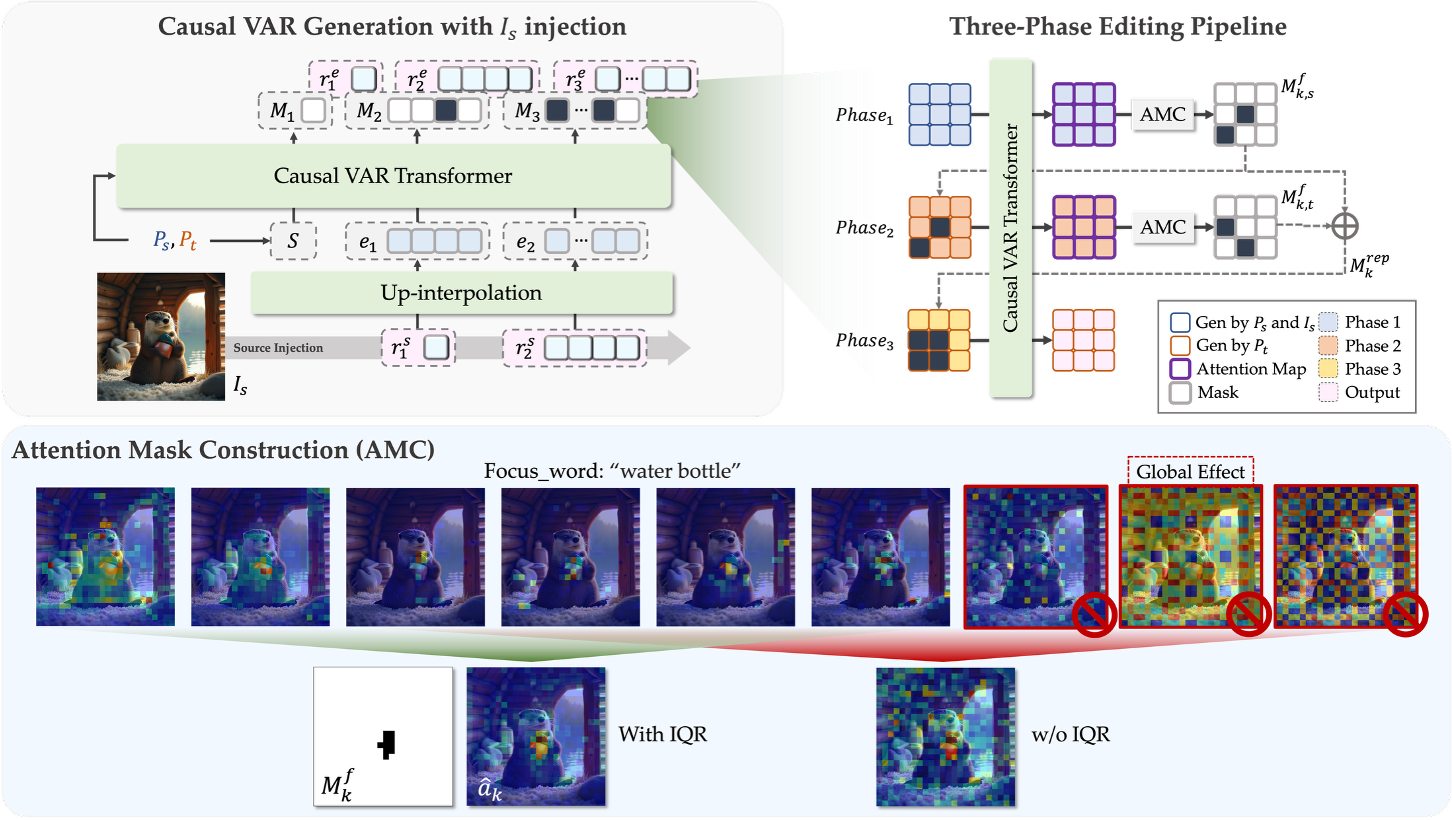
\includegraphics[width=\textwidth]{imgs/pipeline2.png}
    \caption{\textbf{Overview of the proposed editing framework.} \textit{Upper-left:} The source image $I_s$ is encoded into multi-scale discrete tokens $\{r_k^s\}$ via BSQ-VAE; for coarse scales ($k < N$), $r_k^s$ is directly injected into the causal VAR generation to preserve global layout. \textit{Upper-right:} For each scale $k \geq N$, three phases are executed: Phase~1 generates tokens conditioned on $P_s$ to extract $M_{k,s}^{\mathrm{f}}$ and $M_{k,s}^{\mathrm{p}}$; Phase~2 generates tokens conditioned on $P_t$ with background anchoring to extract $M_{k,t}^{\mathrm{f}}$; Phase~3 composes the final output by substituting background positions in $g_k$ with $r_k^s$ according to $M_k^{\mathrm{rep}} = \neg(M_{k,s}^{\mathrm{f}} \cup M_{k,t}^{\mathrm{f}})$. \textit{Bottom:} Detail of Attention Mask Construction (Sec.~\ref{sec:mask_construction}): per-block attention maps $a_{k,b}$ are filtered via IQR to discard positional-bias-dominated transformer blocks, and the retained maps are averaged to produce $\hat{a}_k$, which is then binarized into $M_k^{\mathrm{f}}$ and $M_k^{\mathrm{p}}$.}
    \label{fig:pipeline}
\end{figure*}
   % I.    Introduction
\section{Related Works}
\label{section:3_relatedWorks}
\subsection{Text-Guided Image Editing}
\noindent\textbf{Training-based methods.}
Training-based approaches learn editing capabilities from paired or synthetically constructed datasets. InstructPix2Pix~\cite{InstructPix2Pix} fine-tunes a conditional diffusion model on synthetic instruction--image pairs, enabling single-forward-pass editing from natural language instructions. Imagic~\cite{Imagic} performs complex non-rigid edits by optimizing the text embedding and fine-tuning the model, but requires expensive per-image optimization. BrushNet~\cite{BrushNet} and BrushEdit~\cite{BrushEdit} address region-based inpainting through dual-branch architectures and automated mask generation, respectively. FLUX.1 Kontext~\cite{FLUX.1Kontext} unifies generation and editing by concatenating input and output tokens in latent space with a flow matching objective. While these methods achieve strong editing quality, they face the additional challenge of training overhead and data dependency.
\\
\noindent\textbf{Inversion-based training-free methods.}
A major line of training-free editing relies on inverting a real image into the generative model's latent space. Prompt-to-Prompt (\textit{P2P})~\cite{prompt2prompt} demonstrates that cross-attention maps in diffusion models govern the spatial relationship between image layout and text tokens, enabling localized editing by injecting source attention maps into the target generation process; however, \textit{P2P} operates solely in a text-to-image setting and cannot directly edit real images. Null-text Inversion~\cite{Null-text} addresses this limitation by reconstructing the noise trajectory of an input image through DDIM inversion and optimizing the null-text embedding used in classifier-free guidance. Prompt Tuning Inversion~\cite{Prompt-Tuning} encodes input image information into a learnable conditional embedding via prompt tuning, then interpolates between the optimized and target embeddings to balance editability and fidelity. PnP Inversion~\cite{PnP_Inversion} further simplifies inversion-based editing by rectifying inversion deviations directly within the source diffusion branch while leaving the target branch unaltered. LEDits++~\cite{LEDits++} proposes an efficient perfect inversion scheme with implicit masking that limits changes to semantically relevant regions, supporting multiple simultaneous edits. RF-Inversion~\cite{RF-inversion} extends inversion to rectified flow models by formulating it as dynamic optimal control via a linear quadratic regulator, enabling zero-shot editing for models such as FLUX. Despite progressive improvements, all inversion-based methods remain fundamentally constrained by the accuracy of the inverted trajectory.

\noindent\textbf{Non-inversion training-free methods.}
An alternative line of work avoids explicit inversion altogether. SDEdit~\cite{SDEdit} adds noise to the input image and iteratively denoises through a stochastic differential equation prior, naturally balancing realism and faithfulness but offering limited spatial control. AREdit~\cite{AREdit} is the first to apply training-free editing to Visual Autoregressive Models, caching token indices and probability distributions from the source generation to bridge the information gap between text prompts and the input image. Our method falls in this non-inversion category but differs from AREdit in its editing mechanism: whereas AREdit replays cached token statistics (requiring per-category hyperparameter tuning), we use cross-modal attention maps to explicitly construct spatial editing masks, providing an adaptive and tuning-free alternative.
\subsection{Visual Autoregressive Modeling}
Early discrete visual representation learning established the foundation for autoregressive image generation. VQ-VAE~\cite{VQVAE} introduces vector quantization into the VAE bottleneck, learning discrete latent codes via a straight-through estimator and modeling their distribution with an autoregressive prior; its discrete spatial codes are a conceptual precursor to the token-level editing operations our method performs. VQ-GAN~\cite{VQGAN} extends this by incorporating adversarial training and perceptual losses, producing a perceptually faithful codebook that enables high-resolution image synthesis when combined with an autoregressive transformer over the flattened code grid.
A paradigm shift occurs with VAR~\cite{VAR}, which redefines autoregressive image generation as coarse-to-fine next-scale prediction rather than raster-scan next-token prediction. A multi-scale VQVAE tokenizer encodes images into hierarchical token maps at increasing resolutions, and a transformer autoregressively predicts all tokens at the next finer scale conditioned on coarser scales. This formulation yields substantial improvements in both quality and speed, and demonstrates clear power-law scaling behavior analogous to large language models. Critically for our purposes, the spatial locality of each token---each corresponding to a well-defined patch at a specific scale---is what makes selective token replacement a geometrically meaningful editing operation. HART~\cite{HART} further introduces a hybrid tokenizer that decomposes visual representations into discrete tokens for coarse structure and continuous residual tokens for fine details, with the latter modeled by a lightweight residual diffusion module, bridging the quality gap between discrete autoregressive and continuous diffusion approaches. Infinity~\cite{Infinity} extends VAR by replacing finite-vocabulary codebooks with bitwise token prediction using an infinite-vocabulary tokenizer paired with a bitwise self-correction mechanism, enabling stronger scaling behavior and high-resolution generation. Complementarily, BSQ-VAE~\cite{BSQVAE} proposes Binary Spherical Quantization, a codebook-free approach that projects visual embeddings onto a hypersphere and applies binary quantization, achieving extreme compression with minimal distortion; its lossless encoding property is directly exploited in our framework, where transplanting BSQ-VAE tokens from a source image guarantees pixel-faithful background preservation without any reconstruction distortion.
Our work builds upon the VAR architecture, exploiting two of its structural properties that continuous generative paradigms do not share: the spatial locality of discrete tokens, which enables geometrically precise editing masks, and the self-consistent invertibility of BSQ-VAE encoding, which enables background preservation by construction rather than by approximation.  % II.   Related Work
\section{Preliminaries}
\label{sec:preliminaries}

\noindent\textbf{Visual Autoregressive Modeling.}
Visual AutoRegressive modeling (VAR)~\cite{VAR} redefines image generation as a
coarse-to-fine process: rather than predicting tokens one by one in raster-scan
order, VAR first generates a rough low-resolution representation of the image and
progressively refines it at finer scales. Formally, VAR consists of a multi-scale tokenizer and
an autoregressive transformer. The tokenizer encodes an image $I$ into a hierarchy
of $K$ discrete token maps $\{R_1, R_2, \ldots, R_K\}$ at progressively finer
resolutions, where $R_k \in \mathbb{Z}^{h_k \times w_k}$ and
$h_1 < h_2 < \cdots < h_K$. The transformer then autoregressively predicts the
token map at each subsequent scale conditioned on all coarser scales and text
embeddings $\Psi(t)$:
\begin{equation}
    p(R_1, \ldots, R_K) = \prod_{k=1}^{K} p\!\left(R_k \mid R_1, \ldots,
    R_{k-1},\, \Psi(t)\right)
\end{equation}
All tokens within a scale are predicted in parallel, and each token in $R_k$
corresponds to a spatially well-defined patch at resolution $(h_k, w_k)$. This
spatial locality is the structural property that makes token-level selective
editing geometrically meaningful in our framework.

\noindent\textbf{Infinity and Bitwise Tokenization.}
Infinity~\cite{Infinity} extends VAR by replacing the conventional index-wise
tokenizer with Binary Spherical Quantization (BSQ)~\cite{BSQVAE}, which projects
each continuous residual vector $z_k \in \mathbb{R}^d$ onto the unit hypersphere
and binarizes each dimension:
\begin{equation}
    q_k = \frac{1}{\sqrt{d}}\,\operatorname{sign}\!\left(\frac{z_k}{\|z_k\|}
    \right)
\end{equation}
This formulation scales the vocabulary to effectively infinite size while keeping
computational cost linear in $d$. We adopt Infinity-2B as the backbone of our
framework. Critically for our method, BSQ encoding is \textit{self-consistent}: encoding
a real image into its bitwise token representation and decoding it back introduces
no additional distortion beyond the tokenizer's inherent reconstruction error, meaning that transplanting source tokens into unedited regions
guarantees pixel-faithful background preservation by construction.

\noindent\textbf{Two source-information channels.}
Throughout this paper we distinguish two ways in which the source image enters the
generation process, because they behave very differently. The \textit{continuous}
channel injects the VAE encoder output $\mathcal{E}(I_s)$ (before quantization)
into the accumulated residual maintained across scales, and is used only to
reproduce the source image faithfully while its cross-attention is recorded. The
\textit{discrete} channel supplies the per-scale bitwise tokens
$\{r_k^s\} = \mathcal{Q}_{\mathrm{BSQ}}(\mathcal{E}(I_s))$, and is the only channel
that participates in token substitution. Every token written back into the output
therefore comes from the BSQ quantization of the source image itself, never from an
intermediate generation --- this is what makes background preservation exact rather
than approximate.
 % III.  Preliminaries
%% Eq_methods.tex
%% Simplified equations for Section 4: Methodology
%% Notation: r_k = source tokens at scale k,  A_k = cross-attention map,
%%           a_{k,b} = per-block focus attention,  \hat{a}_k = IQR-filtered attention,
%%           M_k^f = focus mask,  M_k^p = preserve mask,  M_k^rep = replacement mask,
%%           g_k = generated target tokens,  r_k = final output tokens

%% Eq. 1 — BSQ-VAE source image encoding
\newcommand{\EqBsqEncode}{%
\begin{equation}
    \{r_k^s\}_{k=1}^{S} = \mathcal{Q}_{\mathrm{BSQ}}\!\bigl(\mathcal{E}(I_{\mathrm{src}})\bigr),
    \label{eq:bsq_encode}
\end{equation}}

%% Eq. 2 — IQR fence: blocks retained after outlier removal
\newcommand{\EqIqrFilter}{%
\begin{equation}
    \mathcal{B}_{\mathrm{keep}} = \bigl\{ b \;\big|\; e_b \leq Q_3 + 1.5\,(Q_3 - Q_1) \bigr\},
    \label{eq:iqr_filter}
\end{equation}}

%% Eq. 3 — Filtered attention map (mean over retained blocks)
\newcommand{\EqFilteredAttn}{%
\begin{equation}
    \hat{a}_k = \frac{1}{|\mathcal{B}_{\mathrm{keep}}|} \sum_{b \in \mathcal{B}_{\mathrm{keep}}} a_{k,b}.
    \label{eq:filtered_attn}
\end{equation}}

%% Eq. 4a — Min-max normalization of the filtered attention map
\newcommand{\EqNormalize}{%
\begin{equation}
    \tilde{a}_k = \frac{\hat{a}_k - \min \hat{a}_k}{\max \hat{a}_k - \min \hat{a}_k}
    \;\in\; [0,1]^{N_v}.
    \label{eq:normalize}
\end{equation}}

%% Eq. 4b — CV-to-kappa mapping
\newcommand{\EqKappa}{%
\begin{equation}
    \kappa(c_k) = \kappa_{\max}\cdot
    \operatorname{clamp}\!\left(\frac{c_k - c_{\min}}{c_{\max} - c_{\min}},\,0,\,1\right),
    \qquad c_k = \frac{\sigma_k}{\mu_k},
    \label{eq:kappa}
\end{equation}}

%% Eq. 4c — Instance-adaptive threshold on the normalized map
\newcommand{\EqTau}{%
\begin{equation}
    \tau_k = h + \kappa(c_k)\cdot \tilde{\sigma}_k,
    \label{eq:tau}
\end{equation}}

%% Eq. 4d — Focus and preserve masks
\newcommand{\EqMasks}{%
\begin{equation}
\begin{aligned}
    M_k^{\mathrm{f}} &= \mathbf{1}\!\left[\tilde{a}_k \ge \tau_k\right], \\
    M_k^{\mathrm{p}} &= \mathbf{1}\!\left[\tilde{a}_k < \ell\right].
\end{aligned}
\label{eq:masks}
\end{equation}}

%% Eq. 5 — Scale-wise selective token replacement
\newcommand{\EqTokenReplace}{%
\begin{equation}
    r_k = \begin{cases}
        r_k^s & \text{if } k < N \\[2pt]
        M_k^{\mathrm{rep}} \odot r_k^s \;+\; (1{-}M_k^{\mathrm{rep}}) \odot g_k & \text{if } k \geq N
    \end{cases}
    \label{eq:token_replace}
\end{equation}}

%% --- Used in supplementary ---
%% (Coverage ratio equation removed — replaced by adaptive thresholding)

\section{Methodology}
\label{section:method}

\subsection{Overview}
\label{sec:overview}

Given a source image $I_s \in \mathbb{R}^{H \times W \times 3}$, a source prompt $P_s$, and a target prompt $P_t$, the goal of training-free image editing is to produce an edited image $I_e$ that reflects the semantic intent of $P_t$ while preserving all regions not specified by the instruction. Formally:
\begin{equation}
    I_e = f(I_s, P_s, P_t)
\end{equation}
where $f$ is realized entirely at inference time without any parameter updates.

The overall architecture of our proposed method is illustrated in Figure~\ref{fig:pipeline}. The model first resolves spatial editing semantics via cross-modal attention analysis, then selectively rewrites only the targeted tokens. Concretely, our method performs \textbf{dual-stream mask extraction} (Phases~1--2) followed by \textbf{mask-guided token composition} (Phase~3). The edited token map at each scale is:
\begin{equation}
    r_k^e = M_k^{\mathrm{rep}} \odot r_k^s + (1 - M_k^{\mathrm{rep}}) \odot g_k
\end{equation}
where $g_k$ denotes tokens generated under the target prompt, $r_k^s$ the source tokens, and $\odot$ element-wise multiplication. The final edited image $I_e$ is decoded from $\{r_k^e\}_{k=1}^{S}$ by the BSQ-VAE decoder.

\subsection{IQR-Filtered Attention Aggregation}
\label{sec:mask_construction}
\begin{figure}[t]
    \centering
    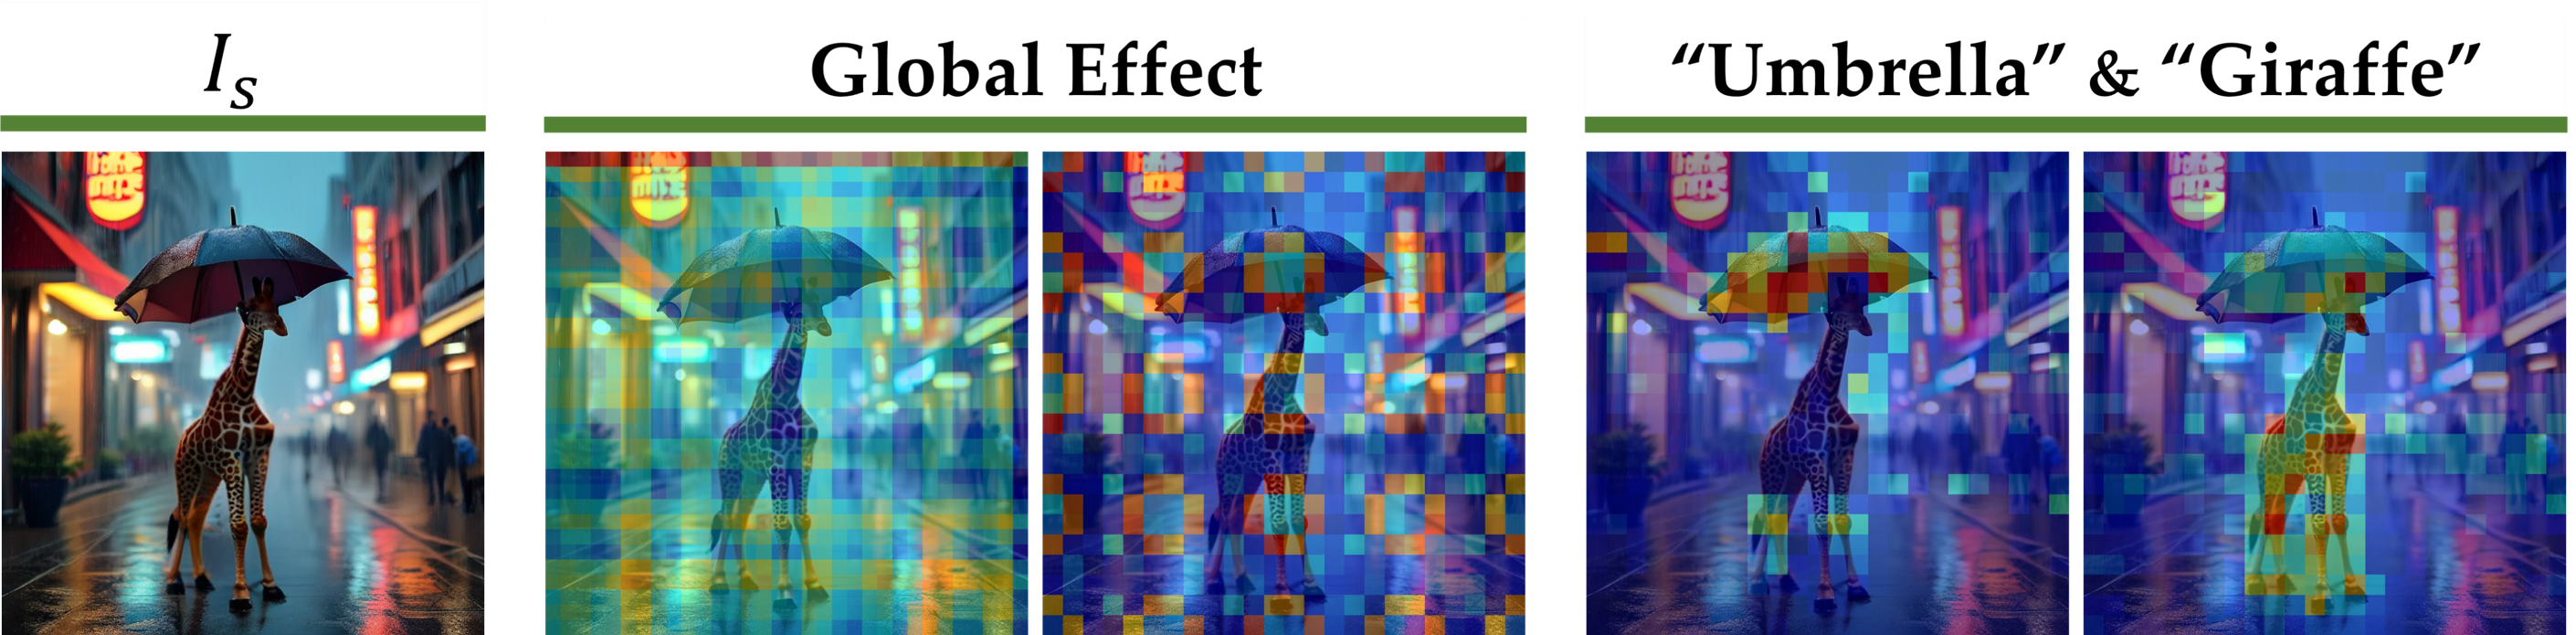
\includegraphics[width=\linewidth]{imgs/globalEffect.png}
    \caption{Global layer effect. \textbf{Middle}: blocks with positional bias produce uniform, non-localizable attention. \textbf{Right}: after IQR filtering, attention correctly focuses on ``Umbrella'' and ``Giraffe''.}
    \label{fig:globalEffect}
\end{figure}

Directly using raw cross-attention maps yields noisy and unreliable masks, because certain transformer blocks produce attention dominated by positional bias rather than semantic content --- a \textit{global layer effect} that spreads attention uniformly regardless of the text query (see Fig.~\ref{fig:globalEffect}).

We suppress these outlier transformer blocks using Interquartile Range (IQR) filtering, a non-parametric method requiring no learned parameters. Let $A_{k,b} \in \mathbb{R}^{N_v \times N_t}$ denote the cross-attention matrix at scale $k$ and transformer block $b$, where $N_v$ is the number of visual tokens and $N_t$ the number of text tokens. Let $\mathcal{F} \subset \{1, \ldots, N_t\}$ denote the set of token indices corresponding to the editing-relevant words in the prompt (e.g., ``water bottle''), identified by differencing the source and target prompts. For each transformer block $b$, we extract the columns of $A_{k,b}$ indexed by $\mathcal{F}$ and average them to obtain a spatial attention map $a_{k,b} \in \mathbb{R}^{N_v}$, which indicates how strongly each visual token attends to the focus words. We then compute the mean attention map across all blocks, $\bar{a}_k = \frac{1}{B}\sum_{b} a_{k,b}$, and measure each block's deviation as $e_b = \mathrm{MSE}(a_{k,b},\, \bar{a}_k)$. Blocks whose deviation exceeds the IQR fence are discarded:
\EqIqrFilter
where $Q_1$ and $Q_3$ are the first and third quartiles of $\{e_b\}$. The retained set $\mathcal{B}_{\mathrm{keep}}$ contains only transformer blocks whose attention maps reflect semantic content rather than positional bias. The filtered attention map is then computed as the mean over the attention maps of these retained blocks:
\EqFilteredAttn
In practice, approximately 10--20\% of blocks are filtered per scale, yielding substantially more spatially coherent attention maps.

\subsection{Instance-Adaptive Mask Binarization}
\label{sec:threshold}

The filtered map $\hat{a}_k$ must be binarized into a focus mask (regions the edit may rewrite) and a preserve mask (background used to anchor source content). This subsection derives the binarization rule, which is the component that most directly controls the preservation--edit trade-off.

\noindent\textbf{Why rank-based thresholds are structurally inadequate.}
A natural first choice is a rank-based rule: take the $p$-th percentile of $\hat{a}_k$ as the threshold. Such a rule, however, \textit{always} selects the top $(1-p)$ fraction of spatial positions, even when the map contains no salient high-energy region at all. This is not a tuning issue but a structural one: for edits such as object addition or global style transfer, the source prompt has no corresponding focus region in the source image, and the correct focus mask may legitimately be empty or near-empty. A rank-based rule cannot express this.

\noindent\textbf{What the attention statistics actually encode.}
A second natural choice is a moment-based threshold $\tau_k = \mu_k + \kappa \sigma_k$, where $\mu_k, \sigma_k$ are the mean and standard deviation of $\hat{a}_k$ and $\kappa$ is modulated by the coefficient of variation $c_k = \sigma_k / \mu_k$ so that concentrated attention yields a tighter mask. Measuring these statistics over the full benchmark, however, reveals that the between-task variation of $c_k$ is driven almost entirely by the \emph{denominator}: across ten editing categories the median $\sigma_k$ spans less than a factor of two, whereas the median $\mu_k$ spans more than a factor of three, in the direction opposite to $c_k$ (Sec.~\ref{sec:cv_analysis}). In other words, $c_k$ is effectively a measure of \textit{how large a fraction of the image the focus region occupies}, and $\mu_k$ --- not the distribution shape --- dominates the absolute scale of $\mu_k + \kappa \sigma_k$. This produces exactly the wrong behaviour in the case that matters most: when the focus word corresponds to a small, well-localized object, attention concentrates on a few positions and the remaining background drags $\mu_k$ down, so $\tau_k$ falls and the resulting mask becomes \emph{larger}.

\noindent\textbf{Absolute-energy threshold with a CV-adaptive correction.}
We therefore decouple the threshold from $\mu_k$ by min-max normalizing the filtered map,
\EqNormalize
and thresholding this normalized energy at an absolute level. The level consists of a fixed base $h$ plus an instance-adaptive correction driven by the coefficient of variation,
\EqKappa
\EqTau
where $\tilde{\sigma}_k$ is the standard deviation of the normalized map $\tilde{a}_k$, and $c_{\min}, c_{\max}, \kappa_{\max}$ define the mapping. The two masks are then
\EqMasks
where $\ell$ is the preserve level. Algorithm~\ref{alg:adaptive_threshold} summarizes the procedure.

\begin{algorithm}[t]
\caption{Instance-Adaptive Mask Binarization}
\label{alg:adaptive_threshold}
\small
\begin{algorithmic}[1]
\Require Filtered attention $\hat{a}_k \in \mathbb{R}^{N_v}$; base level $h$;
         CV range $[c_{\min}, c_{\max}]$; gain $\kappa_{\max}$; preserve level $\ell$
\Ensure Focus mask $M_k^{\mathrm{f}}$, preserve mask $M_k^{\mathrm{p}}$

\State $\mu_k \gets \mathrm{mean}(\hat{a}_k)$,\quad $\sigma_k \gets \mathrm{std}(\hat{a}_k)$
\State $c_k \gets \sigma_k / \mu_k$ \Comment{coefficient of variation, on the \emph{raw} map}
\State $\tilde{a}_k \gets \bigl(\hat{a}_k - \min \hat{a}_k\bigr) / \bigl(\max \hat{a}_k - \min \hat{a}_k\bigr)$
       \Comment{min--max normalization}
\State $\tilde{\sigma}_k \gets \mathrm{std}(\tilde{a}_k)$
\State $\kappa \gets \kappa_{\max}\cdot\operatorname{clamp}\!\bigl((c_k - c_{\min})/(c_{\max} - c_{\min}),\,0,\,1\bigr)$
\State $\tau_k \gets h + \kappa \cdot \tilde{\sigma}_k$ \Comment{$\tau_k \ge h$ since $\kappa \ge 0$}
\State $M_k^{\mathrm{f}} \gets \mathbb{1}[\tilde{a}_k \ge \tau_k]$,\quad
       $M_k^{\mathrm{p}} \gets \mathbb{1}[\tilde{a}_k < \ell]$
\State \Return $M_k^{\mathrm{f}},\, M_k^{\mathrm{p}}$
\end{algorithmic}
\end{algorithm}


Three properties of this formulation are worth making explicit.

\textit{(i) $h$ remains the single semantically meaningful knob.} We fix $\kappa_{\min} = 0$ by construction, so $\tau_k \ge h$ always holds: the adaptive term can only \emph{tighten} the mask relative to the base level, never loosen it. Sweeping $h$ traces a smooth, monotone preservation--edit frontier (Sec.~\ref{sec:frontier}), and the adaptive term shifts that frontier outward rather than adding a second, competing degree of freedom.

\textit{(ii) The focus mask can be empty.} Because the criterion is an absolute energy level rather than a rank, an attention map with no region above $\tau_k$ produces no focus mask, and the corresponding scale is left entirely to source tokens. This is the behaviour a rank-based rule cannot express.

\textit{(iii) The preserve level $\ell$ is not a tuned hyperparameter.} The preserve mask is consumed only by Phase~2, where it anchors background positions to source tokens while the target-side attention is recorded; the tokens generated in that pass are discarded (Sec.~\ref{sec:pipeline}). Consequently $\ell$ influences the final output only through whether the target attention peaks cross $\tau_k$, which it does not affect. We set $\ell = h - 0.01$ throughout.

The parameters $(h, c_{\max}, \kappa_{\max})$ are not hand-tuned; Sec.~\ref{sec:protocol} describes the four-stage protocol used to derive them and reports their sensitivity.
% TODO(verify): confirm against the CLI log of the result directory behind Table I.
% Values used in this paper: h = 0.50, c_min = 0, c_max = 0.20, kappa_min = 0, kappa_max = 0.60.

\subsection{Three-Phase Editing Pipeline}
\label{sec:pipeline}

At each generation scale, the editing pipeline executes three phases in sequence. Phase~1 injects source tokens and extracts source-side masks from cross-attention (see Fig.~\ref{fig:pipeline}), Phase~2 extracts target-side masks with background anchoring, and Phase~3 composes the final tokens by merging the two streams.

\noindent\textbf{Phase~1: Source-Stream Mask Extraction.}
To identify which spatial regions correspond to the source semantics, we generate visual tokens at scale $k$ conditioned on the source prompt $P_s$, with the continuous source features injected at every scale so that the pass reconstructs $I_s$. From the resulting cross-attention, we apply IQR filtering and thresholding (Sec.~\ref{sec:mask_construction}--\ref{sec:threshold}) to obtain the source focus mask $M_{k,s}^{\mathrm{f}}$ and the preserve mask $M_{k,s}^{\mathrm{p}}$.

\noindent\textbf{Phase~2: Target-Stream Mask Extraction.}
Composition needs to know which regions the edit will affect before any token is replaced. Since the source-side mask alone cannot capture regions newly introduced by the target prompt, we perform a second generation pass conditioned on the target prompt $P_t$, anchoring positions where $M_{k,s}^{\mathrm{p}} = 1$ to source tokens $r_k^s$ to prevent background drift. From the resulting cross-attention, we extract the target focus mask $M_{k,t}^{\mathrm{f}}$ via the same filtering and thresholding procedure. The image generated in this pass is discarded; the mask is its only output.

\noindent\textbf{Phase~3: Mask-Guided Token Composition.}
Given the dual-stream masks, we compute the replacement mask $M_k^{\mathrm{rep}} = \neg(M_{k,s}^{\mathrm{f}} \cup M_{k,t}^{\mathrm{f}})$, which marks background positions for source token substitution. We generate the target tokens $g_k$ freely under $P_t$, then assemble the final output:
\EqTokenReplace
Substitution operates on the bitwise token index $r_k \in \{0,1\}^{h_k \times w_k \times d}$, so composition is exact at the bit level and the replaced positions decode to the source content without residual error.

\noindent\textbf{Explicit coarse-scale anchoring.}
For the first $N$ coarse scales, all tokens are replaced with source tokens $r_k^s$ regardless of the masks, because these scales encode the low-frequency global layout. Replacement is strictly binary and the anchoring is explicit rather than folded into a cumulative probability field accumulated over scales, which would inflate the replacement probability at the fine scales and turn the composition into a biased stochastic anchoring. $N$ trades background fidelity against layout freedom; we use $N=2$ throughout.

The complete procedure is summarized in Algorithm~\ref{alg:editing}.

\begin{algorithm}[t]
\caption{Three-Phase Attention-Masked Editing}
\label{alg:editing}
\small
\begin{algorithmic}[1]
\Require Source image $I_{\mathrm{src}}$, prompts $P_s, P_t$, focus word sets $\mathcal{F}_s, \mathcal{F}_t$,
         anchoring scales $N$, total scales $S$
\Ensure Edited image $I_{\mathrm{edit}}$

\State $\{r_k^s\}_{k=1}^{S} \gets \mathcal{Q}_{\mathrm{BSQ}}\!\bigl(\mathcal{E}(I_{\mathrm{src}})\bigr)$
       \Comment{discrete channel}
\State $F_s \gets \mathcal{E}(I_{\mathrm{src}})$ \Comment{continuous channel, Phase~1 only}

\For{$k = 1$ \textbf{to} $S$}

    \Statex \textit{\quad Phase 1: source reconstruction and mask extraction}
    \State Generate tokens at scale $k$ under $P_s$ with $F_s$ injected
    \If{$k \ge N$}
        \State Compute $a_{k,b}$ for $\mathcal{F}_s$; IQR-filter $\to \hat{a}_k^{(s)}$
        \State $M_{k,s}^{\mathrm{f}},\, M_{k,s}^{\mathrm{p}} \gets
               \textsc{AdaptiveBinarize}(\hat{a}_k^{(s)})$ \Comment{Alg.~\ref{alg:adaptive_threshold}}
    \EndIf

    \Statex \textit{\quad Phase 2: target focus mask}
    \State Generate tokens at scale $k$ under $P_t$, anchoring
           $M_{k,s}^{\mathrm{p}}{=}1$ to $r_k^s$
    \If{$k \ge N$}
        \State Compute $a_{k,b}$ for $\mathcal{F}_t$; IQR-filter $\to \hat{a}_k^{(t)}$
        \State $M_{k,t}^{\mathrm{f}},\, \_ \gets
               \textsc{AdaptiveBinarize}(\hat{a}_k^{(t)})$
    \EndIf
    \State \textbf{discard} the tokens generated in Phase~2

    \Statex \textit{\quad Phase 3: composition}
    \State $M_k^{\mathrm{rep}} \gets \neg\!\bigl(M_{k,s}^{\mathrm{f}} \cup M_{k,t}^{\mathrm{f}}\bigr)$
    \State Generate $g_k$ at scale $k$ under $P_t$
    \If{$k < N$}
        \State $r_k \gets r_k^s$ \Comment{explicit coarse anchoring}
    \Else
        \State $r_k \gets M_k^{\mathrm{rep}} \odot r_k^s + (1{-}M_k^{\mathrm{rep}}) \odot g_k$
    \EndIf

\EndFor

\State \Return $\mathcal{D}_{\mathrm{VAE}}\!\bigl(\textstyle\sum_{k} \mathrm{up}(\mathrm{dec}(r_k))\bigr)$
\end{algorithmic}
\end{algorithm}


\noindent\textbf{Text-to-image editing mode.}
Beyond real image editing, our framework naturally extends to a text-to-image (T2I) editing mode by setting $I_s = \varnothing$, i.e., $I_e = f(P_s, P_t)$, where both source and target images are generated from prompts without any real image input. This scenario targets modifying generated content rather than editing an existing photograph. We present T2I editing results and use this mode to validate the attention mask mechanism in Appendix~\ref{app:t2i}.
        % IV.   Methodology
%% ===========================================================================
%%  Section V — Analysis (NEW in the TCSVT version).
%%
%%  ⚠ CONFIG NOTE (must be resolved before submission):
%%  every number in this section comes from the "minimal rewrite + cum0 + N2"
%%  recipe on the full PIE-Bench (700 cases), which is NOT the configuration
%%  behind the main comparison table (tab:method_comparison_wo_kvedit).
%%
%%  Status 2026-08-13: the main-table row cannot be reproduced from anything on
%%  disk.  All 153 summary.json files under outputs/ were scanned; no run comes
%%  close, and no point on the measured frontier attains that row's combination
%%  at once (at SSIM 0.8565 the frontier gives PSNR ~22.1 and LPIPS ~0.092 and IR ~0.73,
%%  against 23.44 / 0.0833 in the table), which suggests the row mixes two runs.
%%  Direct runs of method 15 at the adopted (c_max, k_max) = (0.20, 0.60) give
%%  SSIM 0.8800 / LPIPS 0.0711 / PSNR 23.84 but ImageReward 0.5727.
%%  Decision pending from the author; see TODO.md 5-1.
%%  See ../docs/reports/TCSVT_migration_notes.md §1.
%% ===========================================================================

\section{What Controls the Preservation--Edit Trade-off?}
\label{sec:analysis}

The components introduced in Sec.~\ref{section:method} are not equally
consequential, and several intuitively appealing knobs turn out to have no
effect at all. This section isolates each one on the full benchmark and reports
what actually moves the result and what does not.

\noindent\textbf{Scope of the numbers in this section.}
This section is a controlled comparison, not a second report of our headline
result. Every row here is produced under one common recipe held fixed across the
whole section, and each experiment varies exactly one component of it, so that
rows within the section are comparable to one another and differences can be
attributed. That recipe is deliberately not the configuration of
Table~\ref{tab:method_comparison_wo_kvedit}, which is the single configuration we
report as our method and the only place the reader should read our scores from.
Consequently the absolute values below are not directly comparable to
Table~\ref{tab:method_comparison_wo_kvedit}; only the differences within this
section are. Where a subsection additionally relies on an offline estimate rather
than a direct run, this is stated at that point.

\noindent\textbf{Noise scale.}
Generation is not bit-exact (bf16 kernels with fused attention), so identical
configurations re-run from the same seed differ slightly. Measured over repeated
full-benchmark runs, the run-to-run spread is $\approx\!\pm 0.02$ ImgReward and
$\approx\!\pm 0.001$ HPSv2 at $n{=}700$, widening to $\approx\!\pm 0.05$
ImgReward for a single $n{=}80$ category. We quote this scale whenever a
difference is close to it, and every claim of an effect below is at least three
times it.

\subsection{The Statistics Behind the Threshold}
\label{sec:cv_analysis}

Sec.~\ref{sec:threshold} motivated the absolute-energy criterion by the claim
that the coefficient of variation $c_k$ is driven by the mean rather than the
spread of the attention map. We verify this directly on the last generation
scale ($64\times64$), where the operative masks are built.

Fig.~\ref{fig:cv_decomposition} makes the decomposition explicit.
Across the ten editing categories, the median $c_k$ spans a factor of $4.8$, from $0.31$ for object replacement down to $\approx\!0.067$ for object
addition and style transfer. Decomposing $c_k$ into its numerator and
denominator shows the asymmetry clearly: the median $\sigma_k$ of the ten
categories lies within the narrow band $[0.0008, 0.0017]$ --- less than a factor
of two --- whereas the median $\mu_k$ spans $[0.0049, 0.0157]$, more than a
factor of three, and in the direction \emph{opposite} to $c_k$. The categories
with the lowest $c_k$ are precisely those with the highest $\mu_k$. The signal
that $c_k$ carries is therefore essentially the fraction of the image occupied
by the focus region: when the focus word denotes a small, well-localized object,
attention concentrates on a few positions and the rest of the map approaches
zero, so $\mu_k$ falls and $c_k$ rises; when the focus is a style or a material,
attention spreads over the whole image and $\mu_k$ rises.

This has a direct consequence for a threshold of the form $\mu_k + \kappa
\sigma_k$. Because $\sigma_k \approx \mu_k / 10$ across the benchmark, changing
$\kappa$ over a wide range barely moves the threshold: reducing the mapping from
$\kappa \in [0.5, 1.5]$ to $\kappa \in [0.1, 0.5]$ shifts the median threshold by
only $-9.5\%$. Yet because attention mass is dense just above $\mu_k$, the
induced focus coverage nearly doubles, from $19.4\%$ to $37.9\%$ of the image.
The threshold is thus almost entirely determined by $\mu_k$ --- a per-instance
scale factor that has nothing to do with how selective the mask should be ---
while being extremely sensitive in its effect. Normalizing the map and
thresholding an absolute level (Eq.~\ref{eq:normalize}--\ref{eq:tau}) removes the
$\mu_k$ dependence, which is the entire purpose of the reformulation.

\begin{figure*}[t]
    \centering
    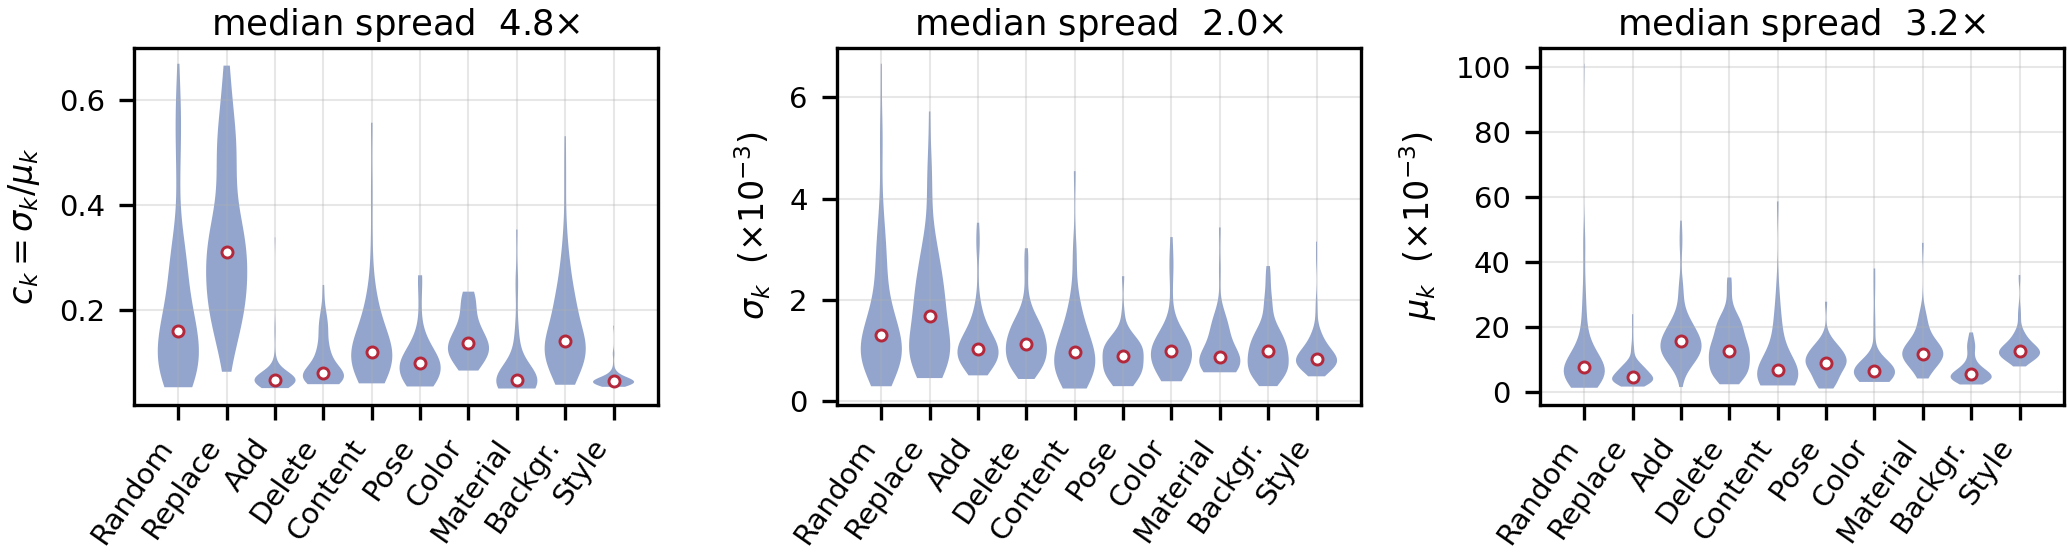
\includegraphics[width=\textwidth]{imgs/fig_cv_decomposition.png}
    \caption{What the coefficient of variation actually measures, over the 700 PIE-Bench cases at the last generation scale ($64{\times}64$). Violins show the per-category distribution; the marker is the median. \textbf{Left:} $c_k$ varies by a factor of $4.8$ between categories. \textbf{Middle:} its numerator $\sigma_k$ varies by only $2.0$. \textbf{Right:} its denominator $\mu_k$ varies by $3.2$, in the direction \emph{opposite} to $c_k$ --- the categories with the lowest $c_k$ (object addition, style transfer) are exactly those with the highest $\mu_k$. The between-category signal in $c_k$ is therefore carried almost entirely by the mean, i.e.\ by how large a fraction of the image the focus region occupies, and not by the shape of the distribution.}
    \label{fig:cv_decomposition}
\end{figure*}


\subsection{$h$ Traces a Smooth Frontier}
\label{sec:frontier}

%% Source: docs/reports/m14_minimal_rewrite_pipeline/ (Table 6) +
%%         docs/reports/m16_candidate_select/ (dense grid, new arms).
%% Recipe: minimal rewrite + cum0 + N2, seed 1, PIE-Bench 700 cases,
%%         kappa_max = 0 (adaptive term disabled, tau = h) so that h is isolated.
%% NOTE: only arms with a complete six-metric record are listed; h = 0.64, 0.65,
%%       0.68, 0.70 exist as runs but are omitted here for compactness.
%% Convention: best in bold, second best underlined, per column.  Note that the
%% two ends of the sweep necessarily take all the marks -- see the caption.
\begin{table}[t]
\centering
\caption{Sweeping the base level $h$ with the adaptive term disabled
($\kappa_{\max}{=}0$, so $\tau_k \equiv h$), which isolates the effect of $h$.
\textbf{Bold} is the best and \uline{underline} the second best in each column,
but here they only mark the two ends of the sweep: this table traces a frontier
rather than comparing alternatives, so no row is ``the'' configuration --- the
point is that every metric is monotone in $h$ and the curve has no
discontinuity. Full PIE-Bench (700 cases).}
\label{tab:frontier_h}
\small
\resizebox{\linewidth}{!}{%
\begin{tabular}{c|cccc|cc}
\toprule
$h$ & S.D.$\downarrow$ & PSNR$\uparrow$ & SSIM$\uparrow$ & LPIPS$\downarrow$ & HPSv2$\uparrow$ & ImgReward$\uparrow$ \\
\midrule
0.48 & 0.0538 & 20.67 & 0.829 & 0.1148 & \textbf{0.2683} & \textbf{0.888} \\
0.50 & 0.0501 & 21.20 & 0.840 & 0.1054 & \uline{0.2651} & \uline{0.818} \\
0.52 & 0.0467 & 21.64 & 0.849 & 0.0978 & 0.2623 & 0.777 \\
0.54 & 0.0432 & 22.18 & 0.859 & 0.0903 & 0.2596 & 0.713 \\
0.56 & 0.0395 & 22.70 & 0.867 & 0.0830 & 0.2569 & 0.645 \\
0.58 & 0.0363 & 23.15 & 0.875 & 0.0771 & 0.2552 & 0.587 \\
0.60 & 0.0331 & 23.66 & 0.882 & 0.0709 & 0.2536 & 0.550 \\
0.62 & 0.0300 & 24.25 & 0.890 & 0.0645 & 0.2517 & 0.466 \\
0.66 & \uline{0.0243} & \uline{25.33} & \uline{0.902} & \uline{0.0547} & 0.2494 & 0.336 \\
0.75 & \textbf{0.0144} & \textbf{27.62} & \textbf{0.921} & \textbf{0.0391} & 0.2489 & 0.096 \\
\bottomrule
\end{tabular}%
}
\end{table}

\begin{figure}[t]
    \centering
    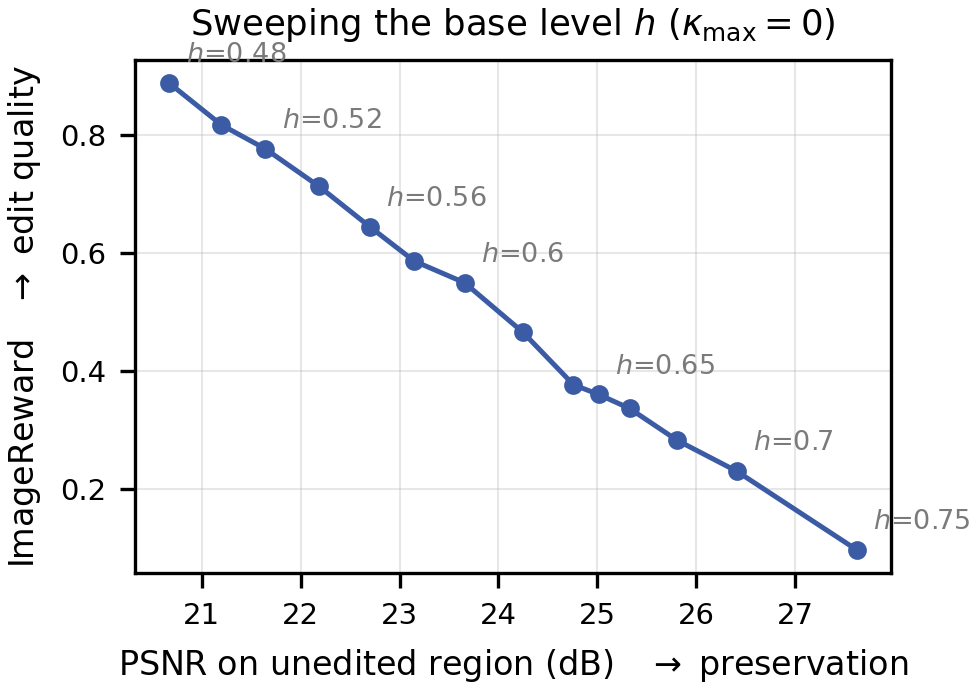
\includegraphics[width=\linewidth]{imgs/fig_frontier_h.png}
    \caption{The base level $h$ traces a smooth, monotone preservation--edit frontier with the adaptive term disabled. Each point is one full-benchmark run (700 cases); $h$ decreases from right to left. Every step of $-0.02$ in $h$ buys roughly $+0.065$ ImageReward for $\approx0.5$\,dB of PSNR, with no discontinuity anywhere in the range.}
    \label{fig:frontier_h}
\end{figure}


Disabling the adaptive term ($\kappa_{\max}{=}0$, so $\tau_k \equiv h$) and
sweeping $h$ over $[0.48, 0.75]$ produces Table~\ref{tab:frontier_h} and
Fig.~\ref{fig:frontier_h}. Every
metric is monotone in $h$ and the curve has no discontinuity anywhere in the
range: each step of $-0.02$ in $h$ buys roughly $+0.065$ ImgReward at a cost of
$\approx\!0.5$\,dB PSNR. Two things follow. First, $h$ is a usable control
surface rather than a value to be tuned once: an application that needs maximal
background fidelity and one that needs aggressive edits select different points
on the same curve, with predictable consequences. Second, because the curve is
smooth, any competing configuration can be compared against it fairly --- one
asks not whether a variant is better, but whether it lies \emph{above} the
frontier. We use this test repeatedly below.

Two properties of the composition rule are fixed once and for all by this test
and are not revisited later. Replacement is strictly binary rather than sampled
from a cumulative probability field accumulated over scales, and the first
$N{=}2$ scales are anchored to source tokens explicitly rather than implicitly;
measured on the same frontier, the two together buy $+1.66$\,dB PSNR and
$-0.013$ LPIPS at unchanged edit strength.

\subsection{The Adaptive Term Shifts the Frontier Outward}
\label{sec:adaptive_gain}

%% Source: docs/reports/m15_param_protocol/report.md, Stage 2 / Stage 4 tables.
%% Dev set = the nine concrete editing categories (n = 560); the mixed category
%% 0_random (n = 140) is excluded from all parameter selection and used only as
%% an independent holdout (see tab:protocol_holdout).
%% Offline evaluation: per-case tau is snapped to the nearest of the 14 h-arms and
%% that arm's per-case scores are read off; used for RELATIVE ranking only.
\begin{table}[t]
\centering
\caption{The CV-adaptive term shifts the frontier outward. At matched
preservation, the adaptive threshold attains a higher edit score than any fixed
threshold on the same frontier (the interpolation of the $\kappa_{\max}{=}0$
arms). Dev set, $n{=}560$.}
\label{tab:adaptive_gain}
\small
\resizebox{\linewidth}{!}{%
\begin{tabular}{l|cccc}
\toprule
Configuration & ImgReward$\uparrow$ & SSIM$\uparrow$ & LPIPS$\downarrow$ & PSNR$\uparrow$ \\
\midrule
\multicolumn{5}{l}{\textit{Fixed threshold ($\kappa_{\max}{=}0$)}}\\
$h = 0.52$ & 0.782 & 0.843 & 0.1023 & 21.17 \\
$h = 0.54$ & 0.724 & 0.853 & 0.0940 & 21.73 \\
\midrule
\multicolumn{5}{l}{\textit{Adaptive threshold}}\\
$(c_{\max}, \kappa_{\max}) = (0.20, 0.60)$ (ours) & 0.734 & 0.856 & 0.0916 & 21.98 \\
$(c_{\max}, \kappa_{\max}) = (0.15, 0.55)$ (grid optimum) & 0.715 & 0.859 & 0.0890 & 22.12 \\
\midrule
\multicolumn{5}{l}{\textit{Gain over the fixed-threshold frontier at matched preservation}}\\
ours @ SSIM $0.856$ & \multicolumn{4}{l}{$0.734$ vs.\ $\approx 0.704$ interpolated \quad $(+0.030)$}\\
ours @ LPIPS $0.0916$ & \multicolumn{4}{l}{$0.734$ vs.\ $\approx 0.702$ interpolated \quad $(+0.032)$}\\
grid opt.\ @ SSIM $0.859$ & \multicolumn{4}{l}{$0.715$ vs.\ $\approx 0.678$ interpolated \quad $(+0.037)$}\\
grid opt.\ @ LPIPS $0.0890$ & \multicolumn{4}{l}{$0.715$ vs.\ $\approx 0.677$ interpolated \quad $(+0.037)$}\\
\bottomrule
\end{tabular}%
}
\end{table}

\begin{figure*}[t]
    \centering
    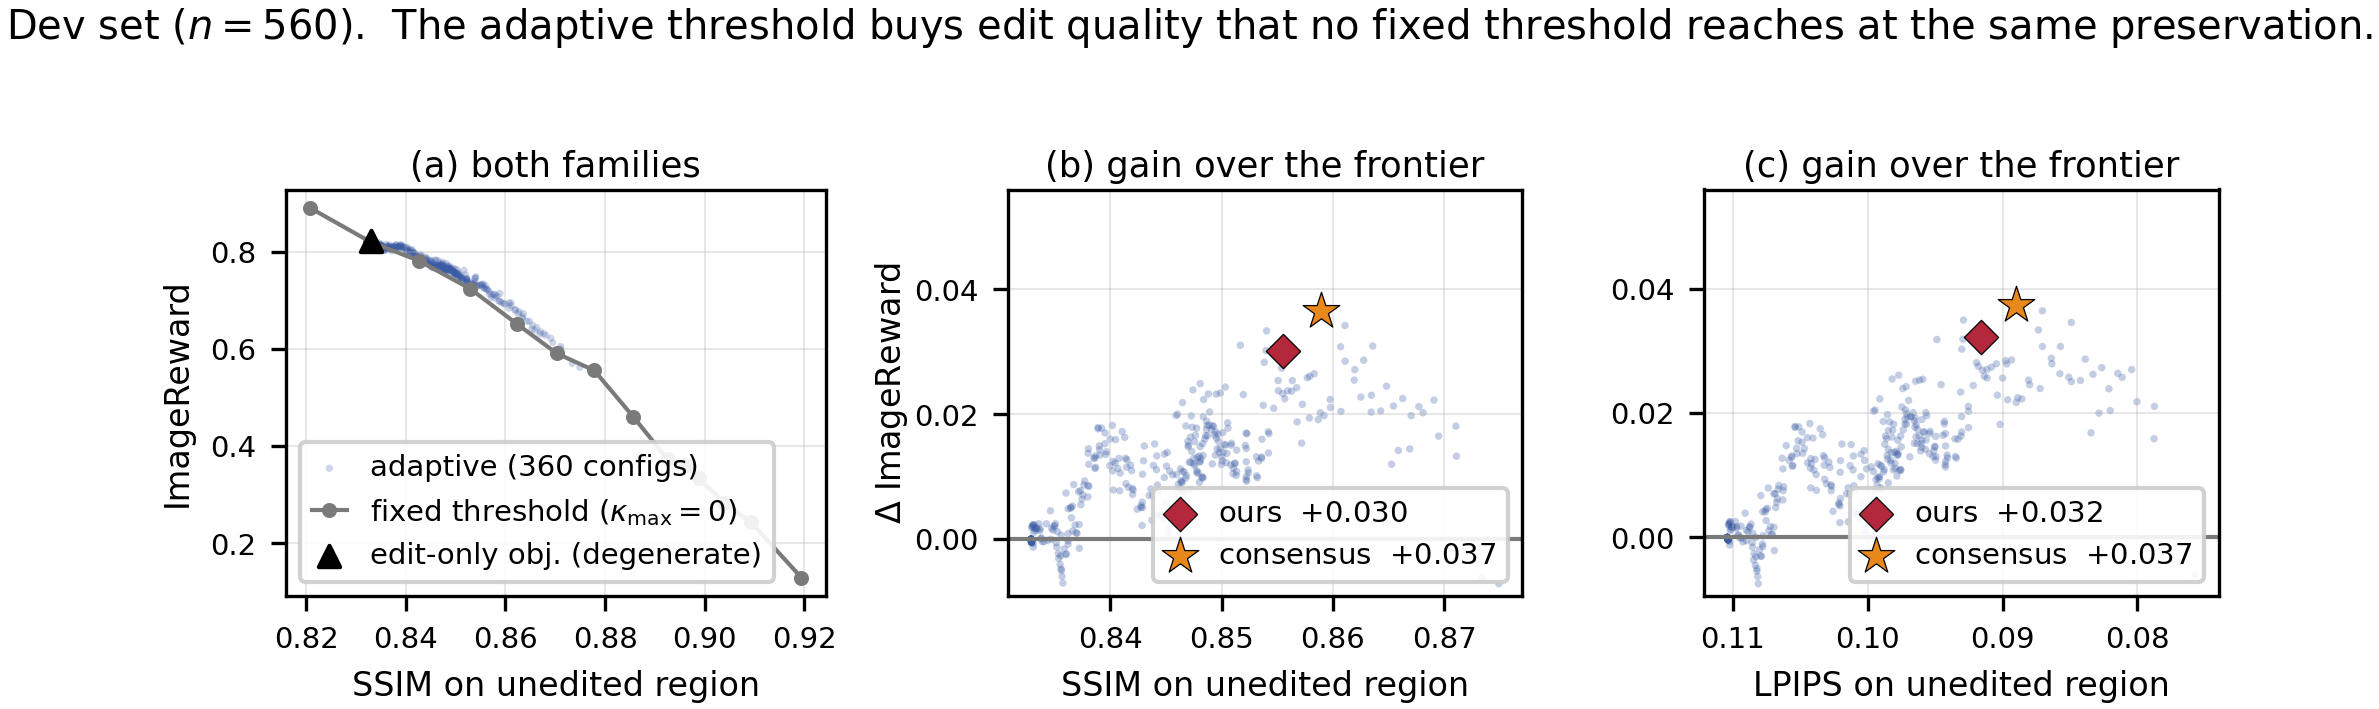
\includegraphics[width=\textwidth]{imgs/fig_adaptive_frontier.png}
    \caption{The adaptive term shifts the frontier outward. \textbf{(a)} The 360 grid configurations of the adaptive threshold against the 14 fixed levels; at this scale the two families are hard to separate, which is why (b) and (c) plot the quantity actually claimed. \textbf{(b, c)} ImageReward of each configuration minus the fixed-threshold frontier \emph{interpolated at the same preservation level}. Positive values are edit quality that no fixed threshold reaches at that preservation. The gain is consistent under two independent preservation metrics: $+0.030$ (SSIM) and $+0.032$ (LPIPS) for the parameters used in this paper, $+0.037$ for the leave-one-category-out consensus. The degenerate edit-only optimum sits on the fixed frontier by construction.}
    \label{fig:adaptive_frontier}
\end{figure*}


A per-instance threshold is only worth its complexity if it beats every fixed
threshold at the same preservation level. Table~\ref{tab:adaptive_gain} performs
that comparison by interpolating the fixed-threshold frontier of
Table~\ref{tab:frontier_h} at the preservation level attained by the adaptive
configuration; Fig.~\ref{fig:adaptive_frontier}(b,\,c) plots the same quantity
for all 360 configurations. Both are offline estimates on the dev set (see the
caveat at the end of Sec.~\ref{sec:protocol}), computed identically for the
adaptive and the fixed arms so that the comparison between them is unaffected.
Direct runs of three adaptive configurations, compared against the fixed
frontier interpolated at the SSIM each of them attains, give ImgReward gains of
$+0.012$, $+0.012$ and $+0.006$. Each of these is inside the run-to-run noise
band quoted above, so on the headline edit metric the adaptive term cannot be
claimed to beat a fixed threshold. The smaller-variance metrics agree in sign
across all three configurations --- HPSv2 $+0.0016$ to $+0.0021$, LPIPS
$-0.0012$ to $-0.0018$, PSNR $+0.24$ to $+0.34$ --- which is consistent with a
real but small effect. We therefore present the adaptive term as a refinement of
the absolute-energy rule, not as a second control surface.
% NOTE: the offline dev-set estimate previously quoted here (+0.030 / +0.037)
% over-states the effect; see docs/reports/m15_scale_dependence/report.md.

The adaptation is also real rather than nominal. Instrumenting a direct run and
recording $\tau_k$ at every scale of every case gives a median of $0.581$ with
interquartile range $[0.549, 0.621]$, spanning most of the usable range of
Table~\ref{tab:frontier_h}. A configuration that merely reproduced a single fixed
threshold under a more complicated formula would show a degenerate distribution
here; this one does not.

The same instrumentation exposes a property of Eq.~\ref{eq:tau} that the
formulation makes easy to overlook: $\tilde{\sigma}_k$ is computed from the
normalized map \emph{at scale $k$}, and it is strongly scale-dependent. Its median
falls monotonically from $0.299$ at the second scale to $0.139$ at the last, so
the same $\kappa$ produces a bump at the coarse scales more than twice the size
of the one it produces at the finest. Because $c_k$ is likewise larger at coarse
scales, $\kappa$ saturates at $\kappa_{\max}$ for $24$--$41\%$ of cases
depending on depth. The threshold is therefore tightest exactly where the layout
is decided, and the induced focus coverage falls from $25\%$ at the second scale
to $5.8\%$ at the last. Any calibration of $(c_{\max}, \kappa_{\max})$ that is
performed on the statistics of a single scale will not transfer to the multi-scale
run; Sec.~\ref{sec:protocol} returns to this.
% TODO(protocol): the four-stage selection below is calibrated on last-scale
% statistics only (sigma_norm ~ 0.138), whereas the run applies the rule at every
% scale (sigma_norm median 0.190).  The selected kappa_max is therefore ~1.4x too
% large in effect.  See docs/reports/m15_scale_dependence/report.md.

\subsection{How the Parameters Were Obtained}
\label{sec:protocol}

%% Source: docs/reports/m15_param_protocol/report.md (Stage 2b, Stage 4);
%% independently reproduced by figs/make_paper_figures.py.
%% dev = 9 concrete editing categories (n=560); holdout = 0_random (n=140),
%% excluded from every stage of parameter selection.
%% Convention: bold = our reported configuration only; no per-column ranking.
\begin{table}[t]
\centering
\caption{Parameter selection. The edit-only optimum collapses to
$\kappa_{\max}\!\to\!0$, i.e.\ back to a fixed threshold, which is why the
selection objective must combine edit quality and preservation
($u = \mathrm{nIR} + \mathrm{nSSIM}$). The selected parameters transfer to a
holdout category that never participated in any stage of the search.
\textbf{Bold} marks our reported configuration in both blocks; no per-column
ranking is marked.}
\label{tab:protocol}
\small
\resizebox{\linewidth}{!}{%
\begin{tabular}{l|cccc|c}
\toprule
Configuration & ImgReward$\uparrow$ & SSIM$\uparrow$ & LPIPS$\downarrow$ & PSNR$\uparrow$ & $\Delta u$ \\
\midrule
\multicolumn{6}{l}{\textit{Dev set: nine editing categories, $n = 560$}}\\
fixed $h{=}0.52$ & 0.782 & 0.843 & 0.1023 & 21.17 & --- \\
fixed $h{=}0.54$ & 0.724 & 0.853 & 0.0940 & 21.73 & --- \\
IR-only optimum $(0.125, 0.05)$ \emph{(degenerate)} & 0.822 & 0.833 & 0.1102 & 20.74 & --- \\
hand-tuned $(0.33, 0.43)$ & 0.772 & 0.846 & 0.0992 & 21.44 & 0.052 \\
\rowcolor{gray!12}
ours $(0.20, 0.60)$ & \textbf{0.734} & \textbf{0.856} & \textbf{0.0916} & \textbf{21.98} & \textbf{0.008} \\
grid optimum $(0.15, 0.55)$ & 0.715 & 0.859 & 0.0890 & 22.12 & 0.000 \\
\midrule
\multicolumn{6}{l}{\textit{Holdout: \texttt{0\_random}, $n = 140$, never used for selection}}\\
fixed $h{=}0.52$ & 0.757 & 0.873 & 0.0817 & 23.33 & --- \\
fixed $h{=}0.54$ & 0.669 & 0.879 & 0.0770 & 23.80 & --- \\
hand-tuned $(0.33, 0.43)$ & 0.708 & 0.877 & 0.0788 & 23.71 & --- \\
\rowcolor{gray!12}
ours $(0.20, 0.60)$ & \textbf{0.657} & \textbf{0.886} & \textbf{0.0720} & \textbf{24.32} & --- \\
grid optimum $(0.15, 0.55)$ & 0.637 & 0.887 & 0.0705 & 24.47 & --- \\
\bottomrule
\end{tabular}%
}

\vspace{2pt}
\raggedright{\footnotesize $\Delta u$ = distance in composite utility from the
grid optimum; the flat region ($u \ge u_{\max} - 0.05$) covers 45\% of the
$18 \times 20$ grid. The leave-one-category-out consensus is $(0.175, 0.55)$,
one grid step away and also inside the flat region.}
\end{table}

\begin{figure*}[t]
    \centering
    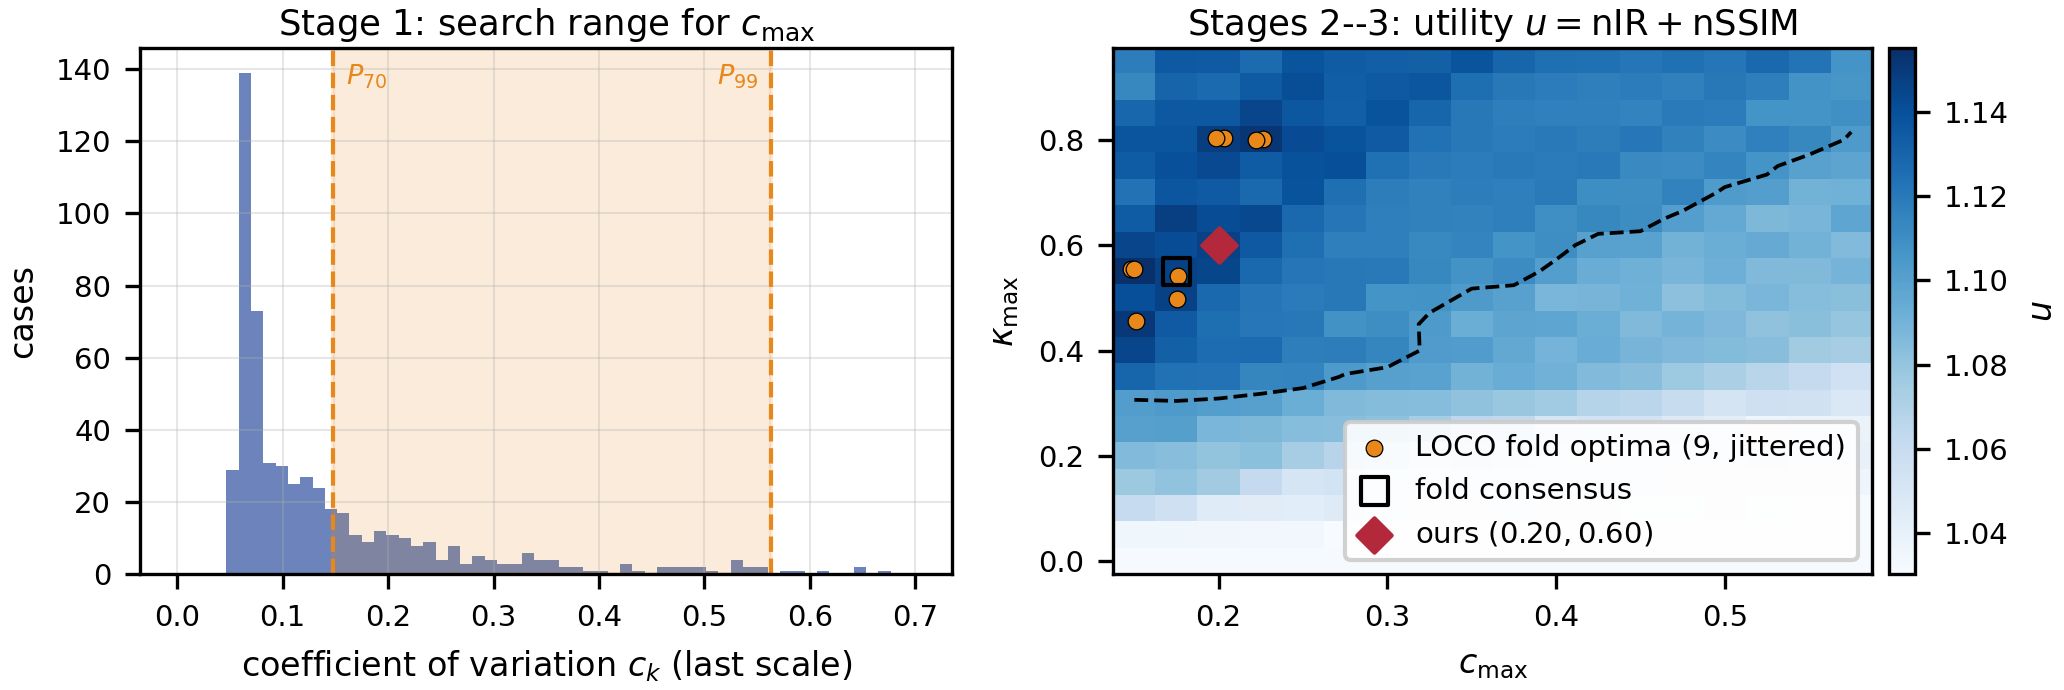
\includegraphics[width=\textwidth]{imgs/fig_protocol.png}
    \caption{Parameter selection. \textbf{Left:} Stage 1 derives the search range for $c_{\max}$ from the dev-set distribution of $c_k$ rather than by hand --- below $P_{70}$ more than half the cases are clamped at $\kappa_{\max}$ and the mapping stops discriminating, above $P_{99}$ nothing is clamped and it degenerates to a linear ramp. \textbf{Right:} the composite utility $u = \mathrm{nIR} + \mathrm{nSSIM}$ over the resulting $18 \times 20$ grid. The dashed contour bounds the flat region ($u \ge u_{\max} - 0.05$), which covers 45\% of the grid; all nine leave-one-category-out optima fall inside it, and the parameters used in this paper sit $\Delta u = 0.008$ from the grid optimum. Utility decreases sharply only towards small $\kappa_{\max}$ (bottom band), i.e.\ the adaptive term has to be given enough range to contribute.}
    \label{fig:protocol}
\end{figure*}


The mapping in Eq.~\ref{eq:kappa} has two free parameters, $c_{\max}$ and
$\kappa_{\max}$. They were not tuned by inspection. We use a four-stage protocol,
run entirely offline on cached attention statistics and per-case scores; the
two stages that involve a choice are shown in Fig.~\ref{fig:protocol}.

\noindent\textit{Stage 1: derive the search space from the data.}
Each boundary is given a statistical meaning rather than a round number. We set
$c_{\max} \in [P_{70}, P_{99}]$ of the dev-set $c_k$ distribution: below $P_{70}$
more than half the cases are clamped at $\kappa_{\max}$ and the mapping ceases to
discriminate, while above $P_{99}$ essentially no case is clamped and the mapping
degenerates to a linear ramp. The upper bound on $\kappa_{\max}$ is obtained by
requiring that the resulting upper threshold not exceed the top of the usable
range identified in Table~\ref{tab:frontier_h}. This yields an $18 \times 20$
grid of $360$ configurations.

\noindent\textit{Stage 2: show that a single-metric objective is degenerate.}
Optimizing mean ImgReward alone selects $\kappa_{\max} \approx 0$
(Table~\ref{tab:protocol}, row 3), reproducing the fixed arm at $h$ to within
$0.001$ IR. This is not a search failure: ImgReward decreases monotonically in
the threshold, so any single-metric objective drives the solution to the lower
boundary of the search space and eliminates the adaptive term entirely. The
objective must therefore combine edit quality and preservation, and we use
$u = \mathrm{nIR} + \mathrm{nSSIM}$ with both terms min-max normalized over the
grid.

\noindent\textit{Stage 3: leave-one-category-out validation.}
Re-running the search on eight categories and validating on the ninth, all nine
folds land inside the flat region of the utility surface, with fold optima
concentrated in $c_{\max} \in [0.150, 0.225]$ and $\kappa_{\max} \in [0.45,
0.80]$. The per-parameter median across folds is $(0.175, 0.55)$, one grid step
from the global optimum $(0.150, 0.55)$ and, like it, well inside the flat
region.

\noindent\textit{Stage 4: sensitivity and holdout.}
The flat region ($u \ge u_{\max} - 0.05$) covers $45\%$ of the grid, so the
selection is not a knife edge; within it, the remaining freedom is a trade-off
preference rather than a performance difference. The parameters used in this
paper sit at $\Delta u = 0.008$ from the grid optimum, inside the flat region and
in the middle of the fold-optima cluster, whereas a hand-chosen setting we used
in early development sits outside it at $\Delta u = 0.052$. Finally, the mixed
category \texttt{0\_random} ($n{=}140$) is excluded from every stage above and
used only as a holdout; the lower block of Table~\ref{tab:protocol} shows the
same ordering there.

\noindent\textbf{Caveat.}
Stages 1--4 evaluate a candidate configuration by snapping each case's threshold
to the nearest of the pre-computed fixed arms and reading that arm's per-case
scores, which makes the $360$-configuration search feasible without any
additional generation. Against a direct run of the same configuration this
offline estimate over-states ImgReward by $\approx\!0.055$ and under-states
preservation, a bias in a consistent direction. We therefore use it only to rank
configurations relative to one another; every number reported outside this
subsection comes from a direct run.
% TODO(rerun): confirm the selected parameters with a direct full-benchmark run
% (scripts/exp_m15_param_consensus.sh) before submission.
      % V.    What controls the preservation-edit trade-off
\section{Experiments}
\label{section:exp}
\begin{table*}[t]
\centering
\caption{Comparison of different editing methods. \textbf{Bold} indicates the
best and \uline{underline} the second best; darker colour indicates better
performance within a column.}
\label{tab:method_comparison_wo_kvedit}
\resizebox{\textwidth}{!}{%
\begin{tabular}{l l c c c c c c c c c c c}
\toprule
Method & Base Model & Param. & S.D.$\downarrow$ & PSNR$\uparrow$ & SSIM$\uparrow$ & LPIPS$\downarrow$ & CLIP whole$\uparrow$ & CLIP edited$\uparrow$ & HPSv2$^{\ddag}\uparrow$ & ImgReward$^{\ddag}\uparrow$ & Resolution & Inf. Time$\downarrow$\\
\midrule
Prompt-to-Prompt \cite{prompt2prompt} & Diffusion & 2B
& \AutoCellDown{0.0694}{0.0222}{0.0694}{0}
& \AutoCellUp{17.87}{17.87}{25.33}{0}
& \AutoCellUp{0.7114}{0.7114}{0.8565}{0}
& \AutoCellDown{0.2088}{0.0833}{0.2088}{0}
& \AutoCellUp{0.2501}{0.2280}{0.2642}{0}
& \AutoCellUp{0.2244}{0.2054}{0.2337}{0}
& \AutoCellUp{0.2592}{0.2035}{0.2931}{0}
& \AutoCellUp{-0.0111}{-0.8649}{0.7344}{0}
& 0.5k
& 13.6 \\

Pix2Pix-Zero \cite{pix2pix-zero} & Diffusion & \textasciitilde1B
& \AutoCellDown{0.0617}{0.0222}{0.0694}{0}
& \AutoCellUp{20.44}{17.87}{25.33}{0}
& \AutoCellUp{0.7467}{0.7114}{0.8565}{0}
& \AutoCellDown{0.1722}{0.0833}{0.2088}{0}
& \AutoCellUp{0.2280}{0.2280}{0.2642}{0}
& \AutoCellUp{0.2054}{0.2054}{0.2337}{0}
& \AutoCellUp{0.2338}{0.2035}{0.2931}{0}
& \AutoCellUp{-0.0375}{-0.8649}{0.7344}{0}
& 0.5k
& 17.0 \\

MasaCtrl \cite{masactrl} & Diffusion & \textasciitilde1B
& \AutoCellDown{0.0284}{0.0222}{0.0694}{0}
& \AutoCellUp{22.17}{17.87}{25.33}{0}
& \AutoCellUp{0.7967}{0.7114}{0.8565}{0}
& \AutoCellDown{0.1066}{0.0833}{0.2088}{0}
& \AutoCellUp{0.2396}{0.2280}{0.2642}{0}
& \AutoCellUp{0.2116}{0.2054}{0.2337}{0}
& \AutoCellUp{0.2399}{0.2035}{0.2931}{0}
& \AutoCellUp{-0.1373}{-0.8649}{0.7344}{0}
& 0.5k
& 12.6 \\

PnP \cite{PnP} & Diffusion & \textasciitilde1B
& \AutoCellDown{0.0282}{0.0222}{0.0694}{0}
& \AutoCellUp{22.28}{17.87}{25.33}{0}
& \AutoCellUp{0.7905}{0.7114}{0.8565}{0}
& \AutoCellDown{0.1134}{0.0833}{0.2088}{0}
& \AutoCellUp{0.2541}{0.2280}{0.2642}{0}
& \AutoCellUp{0.2255}{0.2054}{0.2337}{0}
& \AutoCellUp{0.2644}{0.2035}{0.2931}{0}
& \AutoCellUp{0.3242}{-0.8649}{0.7344}{0}
& 0.5k
& 8.0 \\

PnP Inversion \cite{PnP_Inversion} & Diffusion & \textasciitilde1B
& \AutoCellDown{0.0243}{0.0222}{0.0694}{1}
& \AutoCellUp{22.46}{17.87}{25.33}{0}
& \AutoCellUp{0.7968}{0.7114}{0.8565}{0}
& \AutoCellDown{0.1061}{0.0833}{0.2088}{0}
& \AutoCellUp{0.2541}{0.2280}{0.2642}{0}
& \AutoCellUp{0.2262}{0.2054}{0.2337}{0}
& \AutoCellUp{0.2693}{0.2035}{0.2931}{0}
& \AutoCellUp{0.4111}{-0.8649}{0.7344}{0}
& 0.5k
& 8.0 \\

LEDits++ \cite{LEDits++} & Diffusion & \textasciitilde1B
& \AutoCellDown{0.0431}{0.0222}{0.0694}{0}
& \AutoCellUp{19.64}{17.87}{25.33}{0}
& \AutoCellUp{0.7767}{0.7114}{0.8565}{0}
& \AutoCellDown{0.1334}{0.0833}{0.2088}{0}
& \AutoCellUp{0.2642}{0.2280}{0.2642}{0}
& \AutoCellUp{0.2337}{0.2054}{0.2337}{0}
& \AutoCellUp{0.2035}{0.2035}{0.2931}{0}
& \AutoCellUp{-0.8649}{-0.8649}{0.7344}{0}
& 0.5k
& 2.8 \\
\midrule
FlowEdit \cite{Flowedit} & Flow & 12B
& \AutoCellDown{0.0283}{0.0222}{0.0694}{0}
& \AutoCellUp{21.86}{17.87}{25.33}{0}
& \AutoCellUp{0.8368}{0.7114}{0.8565}{0}
& \AutoCellDown{0.1100}{0.0833}{0.2088}{0}
& \AutoCellUp{0.2605}{0.2280}{0.2642}{0}
& \AutoCellUp{0.2281}{0.2054}{0.2337}{0}
& \AutoCellUp{0.2931}{0.2035}{0.2931}{0}
& \AutoCellUp{0.7229}{-0.8649}{0.7344}{0}
& 0.5k
& 6.5 \\

RF-Inversion \cite{RF-inversion} & Flow & 12B
& \AutoCellDown{0.0406}{0.0222}{0.0694}{0}
& \AutoCellUp{20.82}{17.87}{25.33}{0}
& \AutoCellUp{0.7192}{0.7114}{0.8565}{0}
& \AutoCellDown{0.1900}{0.0833}{0.2088}{0}
& \AutoCellUp{0.2520}{0.2280}{0.2642}{0}
& \AutoCellUp{0.2211}{0.2054}{0.2337}{0}
& \AutoCellUp{0.2847}{0.2035}{0.2931}{1}
& \AutoCellUp{0.5484}{-0.8649}{0.7344}{0}
& 1k
& 24.8 \\

ReFlex \cite{ReFlex} & Flow & 12B
& \AutoCellDown{0.0312}{0.0222}{0.0694}{0}
& \AutoCellUp{25.33}{17.87}{25.33}{0}
& \AutoCellUp{0.8436}{0.7114}{0.8565}{1}
& \AutoCellDown{0.0961}{0.0833}{0.2088}{0}
& \AutoCellUp{0.2602}{0.2280}{0.2642}{0}
& \AutoCellUp{0.2266}{0.2054}{0.2337}{0}
& \AutoCellUp{0.2769}{0.2035}{0.2931}{0}
& \AutoCellUp{0.7334}{-0.8649}{0.7344}{1}
& 1k
& 12.4 \\

FireFlow \cite{FireFlow} & Flow & 12B
& \AutoCellDown{0.0222}{0.0222}{0.0694}{0}
& \AutoCellUp{23.80}{17.87}{25.33}{0}
& \AutoCellUp{0.8211}{0.7114}{0.8565}{0}
& \AutoCellDown{0.1168}{0.0833}{0.2088}{0}
& \AutoCellUp{0.2348}{0.2280}{0.2642}{0}
& \AutoCellUp{0.2084}{0.2054}{0.2337}{0}
& \AutoCellUp{0.2551}{0.2035}{0.2931}{0}
& \AutoCellUp{-0.3778}{-0.8649}{0.7344}{0}
& 0.5k
& 2.5 \\
\midrule
AREdit$^\dag$ \cite{AREdit} & VAR & 2B
& \AutoCellDown{0.0305}{0.0222}{0.0694}{0}
& \AutoCellUp{24.19}{17.87}{25.33}{1}
& \AutoCellUp{0.8370}{0.7114}{0.8565}{0}
& \AutoCellDown{0.0870}{0.0833}{0.2088}{1}
& \AutoCellUp{0.2542}{0.2280}{0.2642}{0}
& \AutoCellUp{0.2277}{0.2054}{0.2337}{0}
& --
& --
& 1k
& 2.5 \\
\rowcolor{gray!10}
Ours & VAR & 2B
& \AutoCellDown{0.0316}{0.0222}{0.0694}{0}
& \AutoCellUp{23.44}{17.87}{25.33}{0}
& \AutoCellUp{0.8565}{0.7114}{0.8565}{0}
& \AutoCellDown{0.0833}{0.0833}{0.2088}{0}
& \AutoCellUp{0.2613}{0.2280}{0.2642}{1}
& \AutoCellUp{0.2290}{0.2054}{0.2337}{1}
& \AutoCellUp{0.2785}{0.2035}{0.2931}{0}
& \AutoCellUp{0.7344}{-0.8649}{0.7344}{0}
& 1k
& 2.5 \\
\bottomrule
\end{tabular}%
}
\vspace{1pt}
\raggedright{\footnotesize $^\dag$Results cited from the original paper; no
official implementation has been released, so HPSv2 and ImageReward cannot be
computed for it.\\
$^\ddag$HPSv2 and ImageReward are human-preference metrics we additionally
measure; they are \emph{not} part of the six official PIE-Bench metrics (S.D.,
PSNR, SSIM, LPIPS, CLIP whole, CLIP edited).}
\end{table*}



\subsection{Experimental Settings}

\noindent\textbf{Benchmark.}
We evaluate on PIE-Bench~\cite{PIEBench}, a comprehensive benchmark comprising 700 images (both natural and artificial) across 10 editing categories, including object replacement, addition, removal, attribute modification, and style transfer.

\noindent\textbf{Metrics.}
Following prior work~\cite{PIEBench,AREdit}, we adopt six metrics grouped into two aspects. For \textit{background preservation}, we report Structure Distance~\cite{PIEBench} (S.D.), PSNR, SSIM, and LPIPS~\cite{LPIPS}. For \textit{editing quality}, we report CLIP similarity~\cite{CLIP} on both the whole image (CLIP whole) and the edited region (CLIP edited). We additionally report two preference models, HPSv2 and ImageReward, which we use throughout Sec.~\ref{sec:analysis}. All metrics are computed using the official PIE-Bench evaluation pipeline; generation is performed at 1k resolution while every metric is computed at $512\times512$ under the standard PIE-Bench protocol. Inference time per image is also reported.

Beyond these six official metrics we additionally measure two \textit{human-preference} models, HPS~v2.1~\cite{hpsv2} and ImageReward~\cite{imagereward}. They are not part of the PIE-Bench metric set; we report them because CLIP similarity measures only image--text alignment and is insensitive both to whether the edit was actually carried out and to whether the result agrees with human preference. One convention has to be stated explicitly: every score we report is computed against the \texttt{editing\_prompt} of the PIE-Bench \texttt{mapping\_file.json}, with its bracket annotations removed. This matters for comparability --- scoring the same images against a paraphrase of that prompt shifts ImageReward by as much as $0.33$, enough to invalidate any comparison that mixes the two conventions. Appendix~\ref{app:eval} documents the full protocol.

\noindent\textbf{Baselines.}
We compare with 11 training-free editing methods spanning three architectural families: six diffusion-based --- Prompt-to-Prompt~\cite{prompt2prompt}, Pix2Pix-Zero~\cite{pix2pix-zero}, MasaCtrl~\cite{masactrl}, PnP~\cite{PnP}, PnP Inversion~\cite{PnP_Inversion}, and LEDits++~\cite{LEDits++} --- four flow-based --- FlowEdit~\cite{Flowedit}, RF-Inversion~\cite{RF-inversion}, ReFlex~\cite{ReFlex}, and FireFlow~\cite{FireFlow} --- and one autoregressive method, AREdit~\cite{AREdit}. Baseline results are obtained using officially released code under default settings, except AREdit whose results are cited directly from the original paper as no official implementation has been released.
% TODO(baselines): add the other VAR-based editors (EditInfinity, BitResEdit,
% VARIN) to this list, to Table I, and to Sec. III; add two columns to Table I
% for mask source (external segmentation / hand-drawn / automatic attention) and
% for whether per-image optimization is required.

\noindent\textbf{Implementation details.}
We build upon Infinity~\cite{Infinity} (2B parameters) with BSQ-VAE~\cite{BSQVAE} ($d{=}32$). Generation uses $S{=}13$ scales ($1{\times}1$ to $64{\times}64$), CFG scale 4.0, and temperature $0.5$. Text conditioning uses Flan-T5-XL~\cite{flan-t5}. We set $N{=}2$ anchoring scales. For mask binarization we use the instance-adaptive threshold of Sec.~\ref{sec:threshold} with $h{=}0.50$, $c_{\min}{=}0$, $c_{\max}{=}0.33$, $\kappa_{\min}{=}0$, $\kappa_{\max}{=}0.43$ and $\ell = h - 0.01 = 0.49$; Sec.~\ref{sec:calibration} describes how they are obtained. For IQR filtering, we discard transformer blocks whose attention deviation from the cross-block mean exceeds the IQR fence (Sec.~\ref{sec:mask_construction}), using blocks 2--31 of the 32-block model (blocks 0--1 are excluded as they consistently exhibit the global attention effect described in Sec.~\ref{sec:mask_construction}). All experiments run on a single NVIDIA RTX 5090 GPU with ${\sim}$2.5\,s inference per image.
%% Verified 2026-08-13 against the run behind the main table:
%% pie_edit_rewrite_minimal_m15_h0.50_k0-0.43_cum0_N2 (method 15, h=0.50,
%% cv[0,0.33], kappa[0,0.43], l=0.49, cum0, N=2, minimal rewrite, seed 1, n=700).
%% Measured runtime tau median 0.537 over all scales.

\subsection{Comparison with State-of-the-Art Methods}

\noindent\textbf{Quantitative results.}
Table~\ref{tab:method_comparison_wo_kvedit} summarizes the comparison. Our
method attains the best SSIM ($0.8565$) and LPIPS ($0.0833$) of any method
compared, and the second-best CLIP whole ($0.2613$) and CLIP edited ($0.2290$),
showing strong background preservation together with competitive edit quality
from a 2B backbone --- one sixth of the parameters of every flow-based baseline.
We are not best on Structure Distance or PSNR, and this reflects the choice of
operating point: as Sec.~\ref{sec:frontier} shows, background preservation and
edit strength trade off along a continuous frontier, and we select a point that
balances the two.

\noindent\textbf{Human-preference metrics.}
On the two additional preference metrics our ImageReward is $0.7344$, essentially
identical to the closest baseline ReFlex ($0.7334$); the gap of $0.001$ is far
below the full-benchmark run-to-run spread (about $\pm 0.02$,
Sec.~\ref{sec:analysis}), so the two should be read as \textit{level} rather
than as a lead. The substantive conclusion on ImageReward is that we are on par
with two 12B flow-based models (ReFlex, and FlowEdit at $0.7229$) with one sixth
of their parameters. On HPSv2 we reach $0.2785$, third behind FlowEdit
($0.2931$) and RF-Inversion ($0.2847$). No official implementation of AREdit has
been released, so we cannot obtain its outputs and cannot compute either metric
for it.

\textit{vs.\ diffusion-based methods.}
Compared to the best diffusion-based method PnP Inversion, we improve SSIM by $7.5\%$ and LPIPS by $21.5\%$ while achieving higher CLIP scores on both whole-image and edited-region metrics.

\textit{vs.\ flow-based methods.}
Against the strongest flow-based competitor ReFlex, we attain better SSIM and
LPIPS despite the $6\times$ parameter gap, though ReFlex achieves higher PSNR.

\textit{vs.\ AREdit.}
AREdit~\cite{AREdit} is the closest comparison: a training-free editor on the same 2B VAR backbone. We are better on SSIM, LPIPS and both CLIP metrics, while AREdit is slightly ahead on Structure Distance and PSNR. The more consequential difference is where the mask comes from: AREdit requires the user to supply a threshold per editing category, whereas our masks are derived entirely from the model's own cross-attention with no per-category tuning --- which is precisely the advantage of attention-driven mask construction over cached token statistics.
% TODO(optional): if Table I gains a preservation-oriented row, quote it here.
% A higher-h operating point under this formulation reaches PSNR/S.D. comparable
% to or better than AREdit; that row must come from a direct run under the SAME
% configuration as the rest of Table I before it can be quoted.

We report inference time for reference, but note that methods operate at different generation resolutions; all metrics are nevertheless computed at the common $512\times512$ evaluation resolution.

\begin{figure*}[!t]
    \centering
    \includegraphics[width=\textwidth]{imgs/qualitative.png}
    \caption{Qualitative comparison with FireFlow, FlowEdit, ReFlex, RF-Inversion, LEDits++, MasaCtrl, PnP, and PnP-Inversion across diverse editing types: attribute replacement (smoke$\to$fire), pose change (sitting$\to$standing), object addition (+flowers), and style transfer (watercolor$\to$anime). Notably, the second row shows that our method correctly transforms the bear's pose from sitting to standing while preserving both the background and the bear's visual identity. More results are provided in the appendix.}
    \label{fig:qualitative}
\end{figure*}

\noindent\textbf{Qualitative results.}
Fig.~\ref{fig:qualitative} presents representative visual comparisons. Diffusion-based methods often suffer from structural drift or incomplete edits due to inversion errors: P2P and Pix2Pix-Zero alter the global layout, while MasaCtrl preserves structure but produces blurry edited regions. Among flow-based methods, ReFlex achieves the best preservation but occasionally misses fine-grained edit details. In contrast, our method produces clean, precisely localized edits while faithfully preserving the background, benefiting from explicit attention-driven masking and discrete token replacement.

\subsection{Attention Masking vs.\ Scale-Level Replacement}
\label{sec:ablation_mask}

The most basic alternative to a spatial mask is no spatial mask at all: share the first $N$ scales with the source by full replacement and let every later scale generate freely under $P_t$. We denote this variant Scale-$N$ and vary $N \in \{1, 2, 4, 6\}$.

%% Convention: best in bold.
\begin{table}[t]
\caption{Ablation on attention-based masking. \emph{Scale-$N$}: the first $N$
scales are replaced with source tokens and no attention mask is applied at any
later scale. \emph{Attn Mask}: the full three-phase pipeline. S.D.\ is Structure
Distance. \textbf{Bold} is the best.}
\label{tab:ablation_mask}
\centering
\small
\resizebox{\linewidth}{!}{%
\begin{tabular}{l|cccc|cc}
\toprule
Config & S.D.$\downarrow$ & PSNR$\uparrow$ & SSIM$\uparrow$ & LPIPS$\downarrow$ & CLIPw$\uparrow$ & CLIPe$\uparrow$ \\
\midrule
Scale-1 & 0.0843 & 12.25 & 0.4330 & 0.3930 & 0.2439 & 0.2210 \\
Scale-2 & 0.0807 & 12.56 & 0.4450 & 0.3810 & 0.2427 & 0.2199 \\
Scale-4 & 0.0611 & 14.08 & 0.4960 & 0.3190 & 0.2121 & 0.1946 \\
Scale-6 & 0.0424 & 15.66 & 0.5530 & 0.2560 & 0.2001 & 0.1822 \\
\midrule
Attn Mask (Ours) & \textbf{0.0316} & \textbf{23.44} & \textbf{0.8565} & \textbf{0.0833} & \textbf{0.2613} & \textbf{0.2290} \\
\bottomrule
\end{tabular}}
\end{table}

\begin{figure}[t]
    \centering
    \begin{subfigure}[t]{1\linewidth}
        \centering
        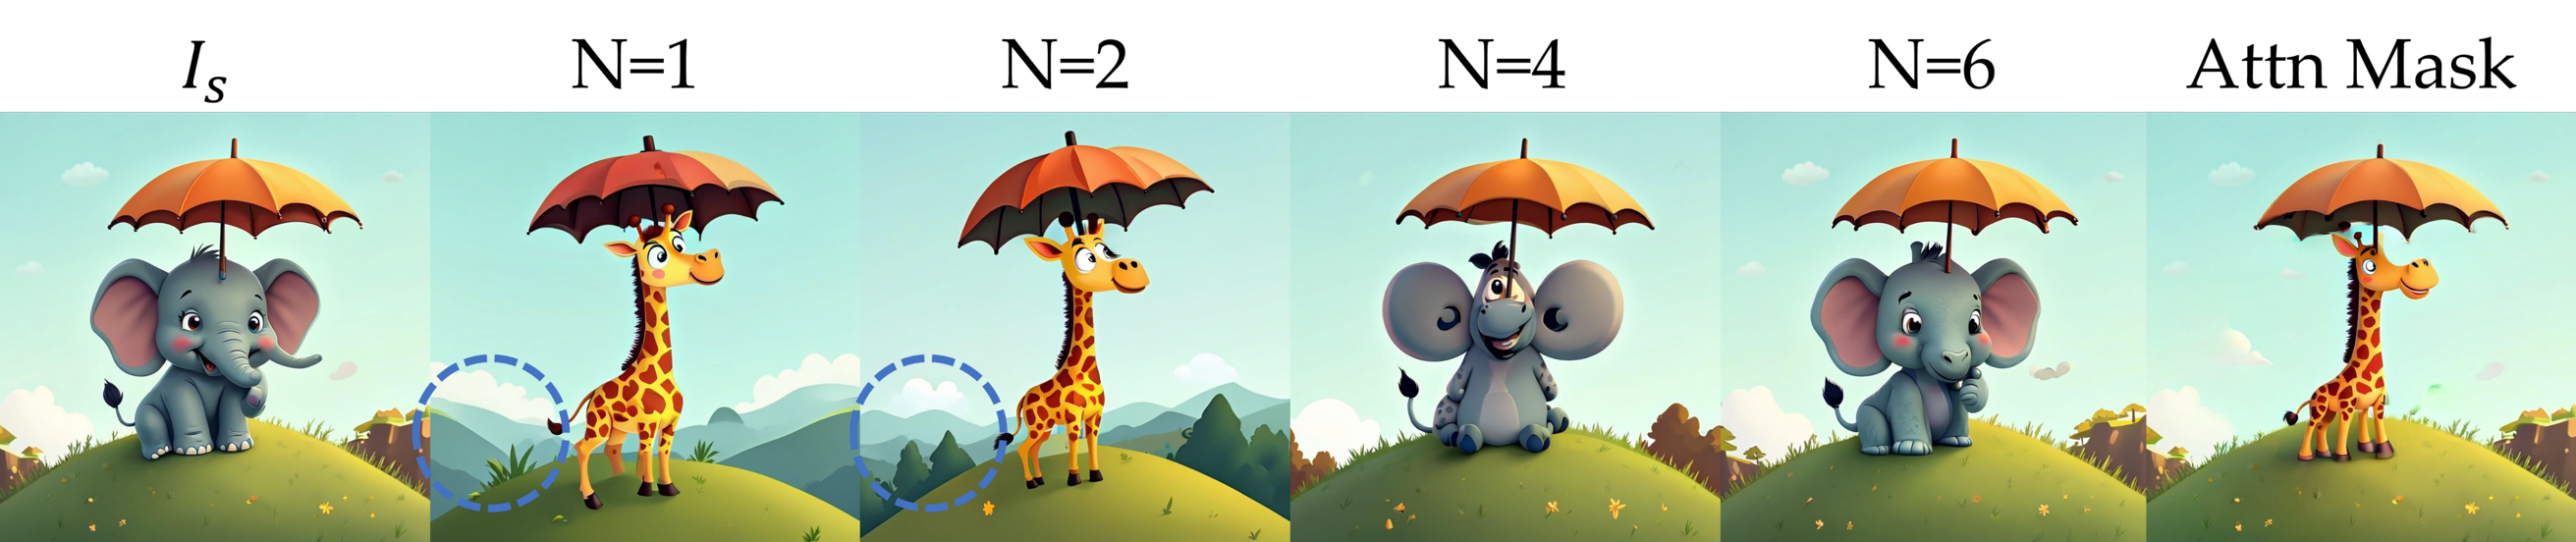
\includegraphics[width=\linewidth]{imgs/shape_diff.png}
        \caption{Scale-$N$ replacement: few shared scales allow editing but lose the background; many shared scales preserve the background but lock the subject. Our attention-mask approach achieves both precise editing and faithful preservation.}
        \label{fig:shape_diff_a}
    \end{subfigure}
    \hfill
    \begin{subfigure}[t]{1\linewidth}
        \centering
        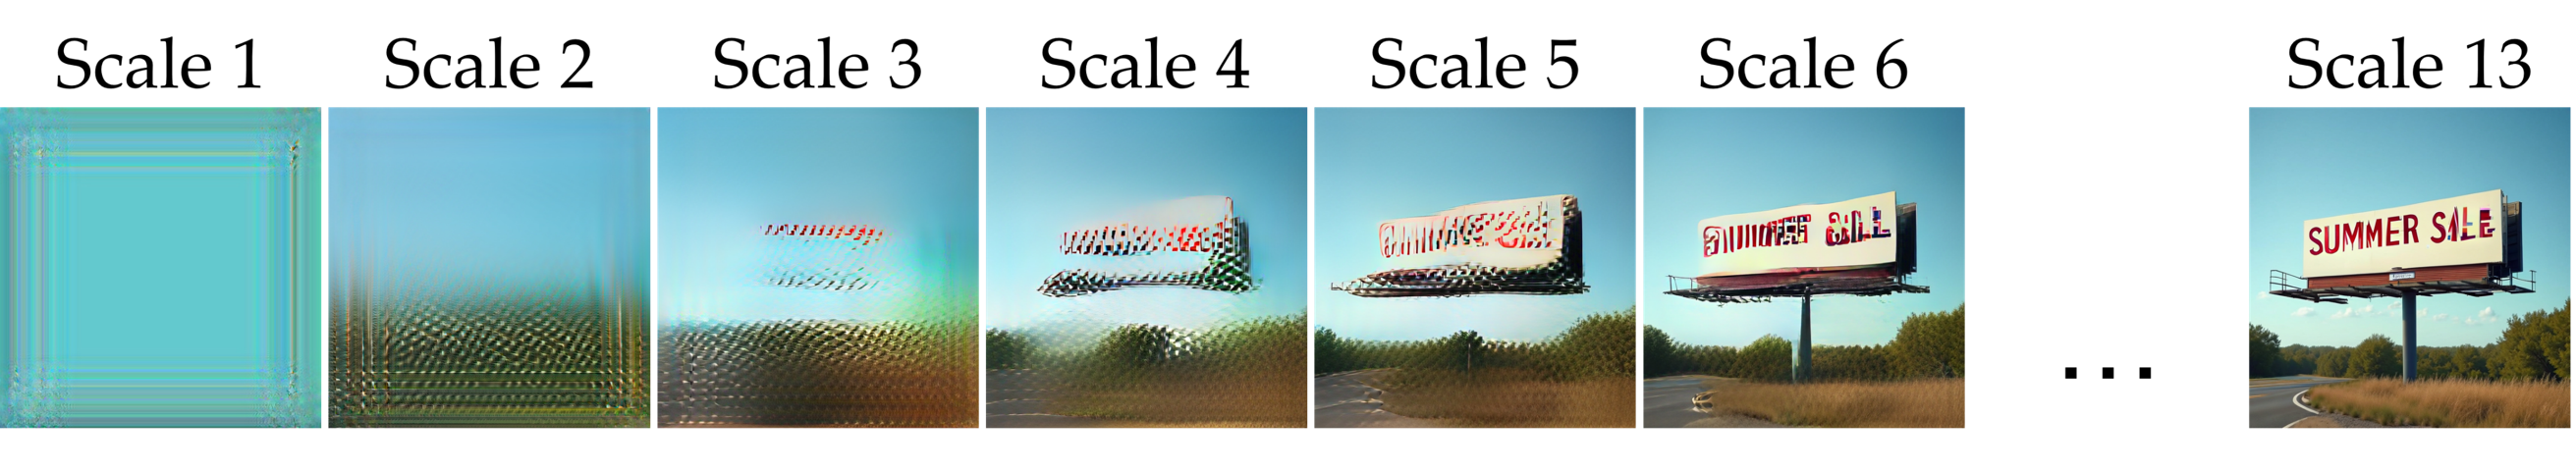
\includegraphics[width=\linewidth]{imgs/coarse2fine.png}
        \caption{VAR's coarse-to-fine generation: early scales ($k \leq 4$) determine global layout; later scales refine texture. Fixed-scale replacement thus cannot accommodate shape-changing edits.}
        \label{fig:shape_diff_b}
    \end{subfigure}
    \caption{Analysis of scale-level replacement vs.\ attention-based masking. (a) Comparison across configurations on an elephant $\to$ giraffe edit. (b) VAR's coarse-to-fine generation: early scales commit to global layout, limiting the effectiveness of fixed-scale replacement strategies.}
    \label{fig:shape_diff}
\end{figure}

As shown in Table~\ref{tab:ablation_mask}, increasing the number of shared scales progressively improves preservation, but the gains saturate: even at $N{=}6$ --- nearly half of the 13 scales --- SSIM reaches only $0.553$, because every scale beyond $N$ generates with no reference to the source. Per-token spatial guidance at every scale improves SSIM by 55\% and LPIPS by 67.5\% over the best Scale-$N$ variant.

Fig.~\ref{fig:shape_diff} explains why the saturation is structural rather than a matter of choosing $N$ better. Fig.~\ref{fig:shape_diff_a} shows the two failure modes at the ends of the range: few shared scales permit the edit but destroy the background, while many shared scales preserve the background and simultaneously lock the subject, since the global layout is already committed. Fig.~\ref{fig:shape_diff_b} shows the underlying cause --- VAR fixes the global arrangement within the first few scales and spends the remainder on texture --- so a shape-changing edit must modify early tokens, which uniform scale-level replacement cannot do selectively. Attention masking resolves the tension by replacing only background positions at every scale, which is what makes precise editing and faithful preservation simultaneously attainable. The residual cost of the coarse anchoring that remains is analyzed in Sec.~\ref{sec:limitations}.

\subsection{Phase 2}
\label{sec:ablation_phase2}

Phase~2 performs a second generation pass under the target prompt in order to
extract the target focus mask $M_{k,t}^{\mathrm{f}}$ before any token is replaced
(Sec.~\ref{sec:pipeline}). We compare the full three-phase pipeline against a
variant that skips Phase~2 entirely.

%% Translated from NTUST_Thesis_Kai/tabs/ablationPhase2.tex.
%% Simple two-arm ablation: the full three-phase pipeline versus the same
%% pipeline with Phase 2 skipped entirely.
%% Convention: best in bold (two rows only, so no second-best mark).
\begin{table}[t]
\centering
\caption{Ablation of Phase~2. \textbf{Bold} is the best.}
\label{tab:ablation_phase2}
\small
\resizebox{\linewidth}{!}{%
\begin{tabular}{l|cccc|cc}
\toprule
Method & S.D.$\downarrow$ & PSNR$\uparrow$ & SSIM$\uparrow$ & LPIPS$\downarrow$ & CLIPw$\uparrow$ & CLIPe$\uparrow$ \\
\midrule
With Phase 2 & \textbf{0.0316} & \textbf{23.44} & \textbf{0.8565} & \textbf{0.0833} & \textbf{0.2613} & \textbf{0.2290} \\
W/O Phase 2  & 0.0518 & 17.02 & 0.6228 & 0.2047 & 0.2522 & 0.2212 \\
\bottomrule
\end{tabular}%
}
\end{table}


As shown in Table~\ref{tab:ablation_phase2}, Phase~2 is the single largest
contribution of any component: PSNR improves by $37.7\%$, SSIM by $37.5\%$,
LPIPS drops by $59.3\%$ and Structure Distance by $39.0\%$, with the CLIP scores
also rising by $3.5$--$3.6\%$. These results confirm that a source-side mask alone
cannot delineate the edit boundary accurately --- least of all when the target
introduces spatial content that does not exist in the source. The dual-stream
mask construction of Phases~1--2 is therefore indispensable for achieving precise
edits without background drift.

\subsection{IQR Filtering}
\label{sec:ablation_iqr}

Not all transformer blocks produce equally informative attention maps. As described in Sec.~\ref{sec:mask_construction}, we measure each block's deviation from the cross-block mean and discard outlier blocks whose deviation exceeds the IQR fence. We compare our full model against naively averaging all blocks.

%% Split out from the old tabs/ablationThreshold.tex: only the IQR part remains
%% here, since the "adaptive vs fixed percentile" comparison belonged to the
%% rank-based formulation and is superseded by Sec. V-B / V-C.
\begin{table}[t]
\centering
\caption{Ablation on IQR block filtering. Removing the filter and averaging all
blocks lets positional-bias-dominated attention corrupt the mask. Both rows are
measured under one common configuration held fixed across the ablation, which is
not the operating point reported in
Table~\ref{tab:method_comparison_wo_kvedit}; the comparison between rows is
unaffected. Nothing is marked.}
\label{tab:ablation_iqr}
\small
\resizebox{\linewidth}{!}{%
\begin{tabular}{l|cccc|cc}
\toprule
Method & S.D.$\downarrow$ & PSNR$\uparrow$ & SSIM$\uparrow$ & LPIPS$\downarrow$ & CLIPw$\uparrow$ & CLIPe$\uparrow$ \\
\midrule
\rowcolor{gray!12}
With IQR & 0.0316 & 23.44 & 0.8565 & 0.0833 & 0.2613 & 0.2290 \\
W/O IQR   & 0.0328 & 20.56 & 0.7872 & 0.1285 & 0.2550 & 0.2260 \\
\bottomrule
\end{tabular}%
}
\end{table}

% \begin{figure}[t]
%     \centering
%     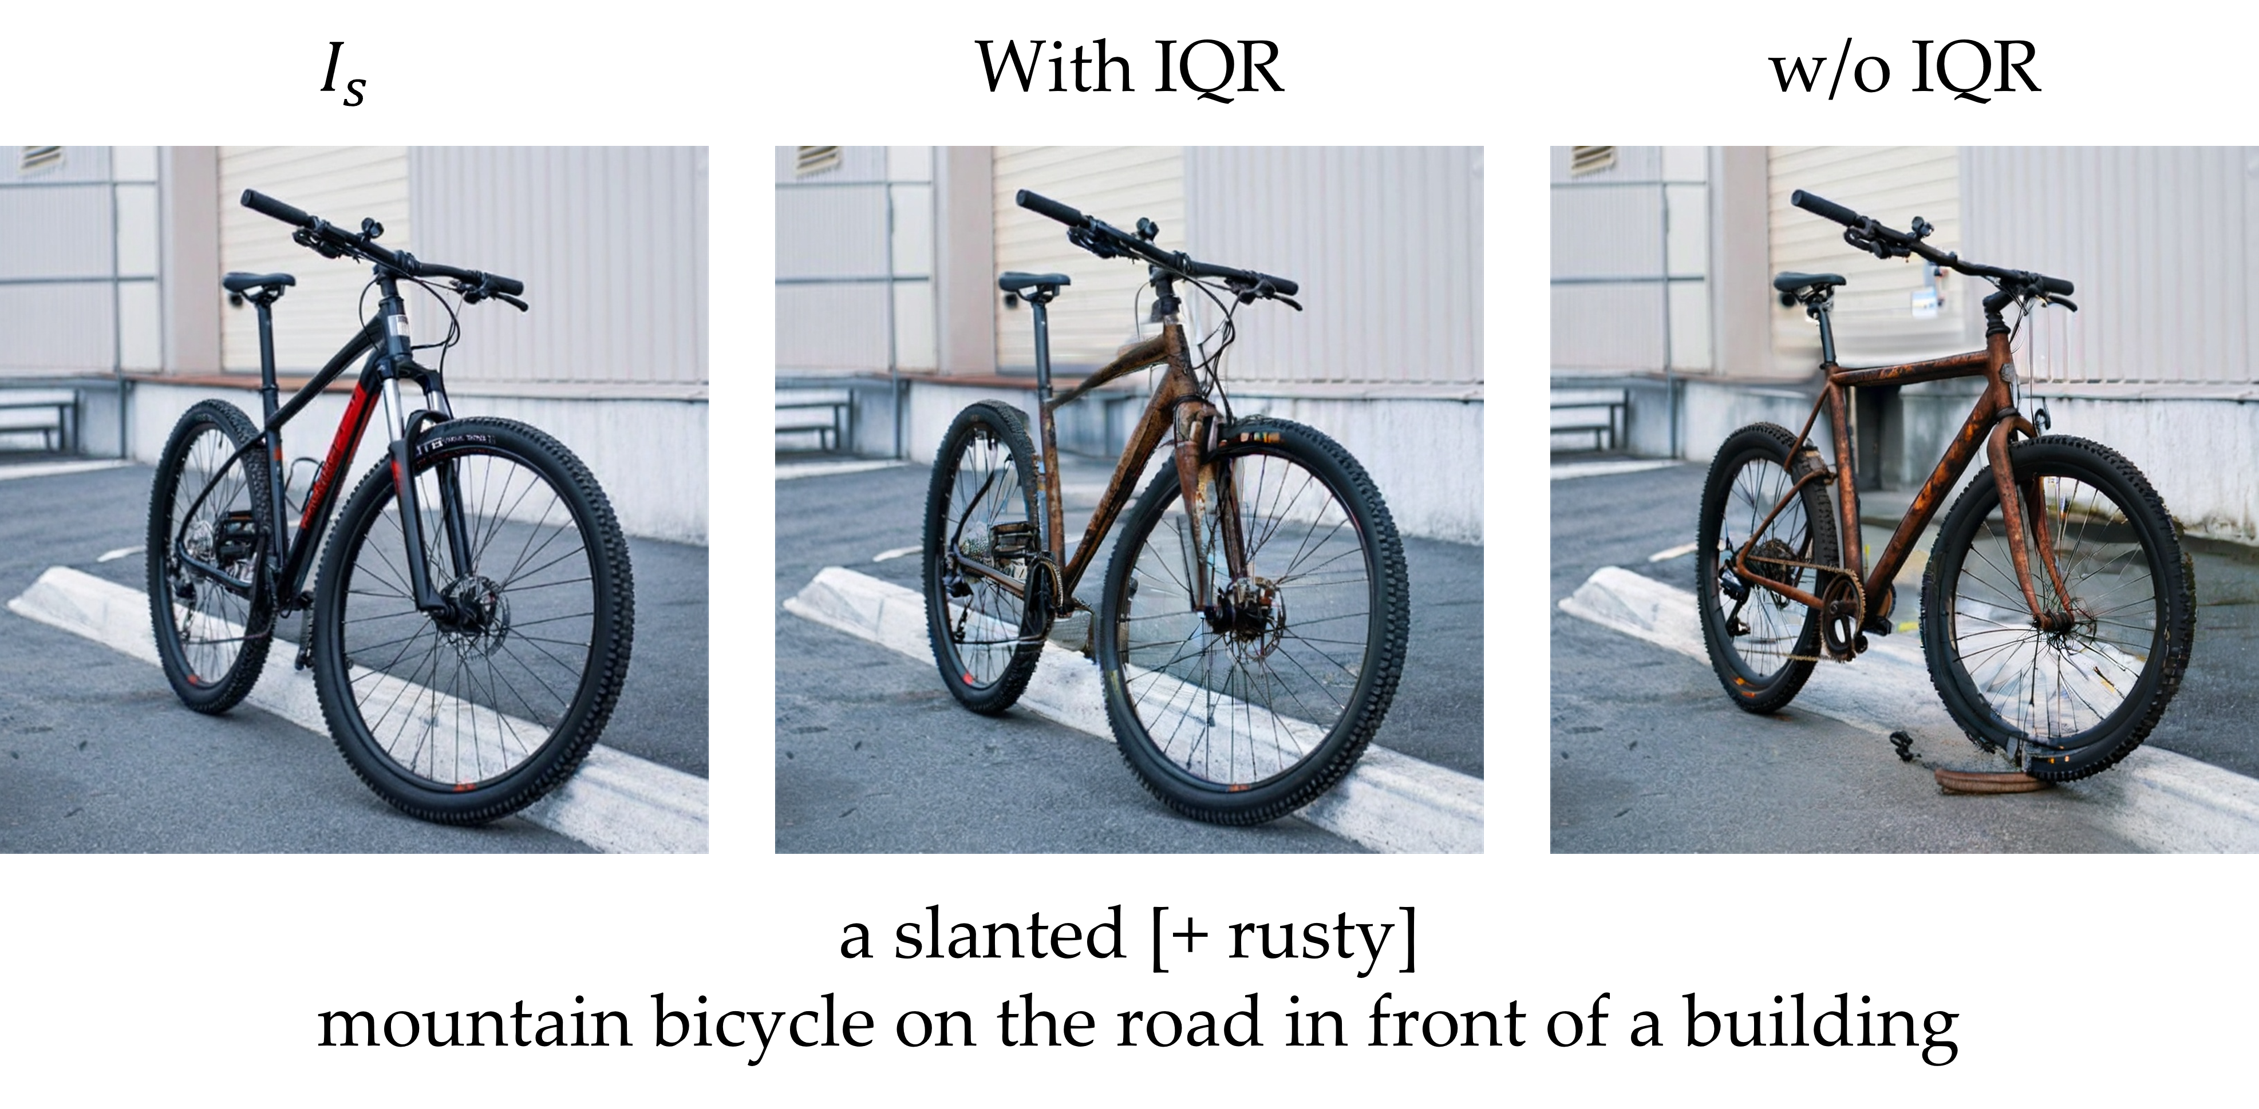
\includegraphics[width=\linewidth]{imgs/ablationIQR.png}
%     \caption{Effect of IQR filtering on editing quality. $I_s$ denotes the source image. With IQR filtering, the generated mask accurately captures the editing region, preserving the overall structure of the bicycle. Without IQR filtering, the bicycle structure is severely distorted, demonstrating that IQR-based block selection is critical for producing reliable attention masks.}
%     \label{fig:ablationIQR}
% \end{figure}
\begin{figure}[t]
    \centering
    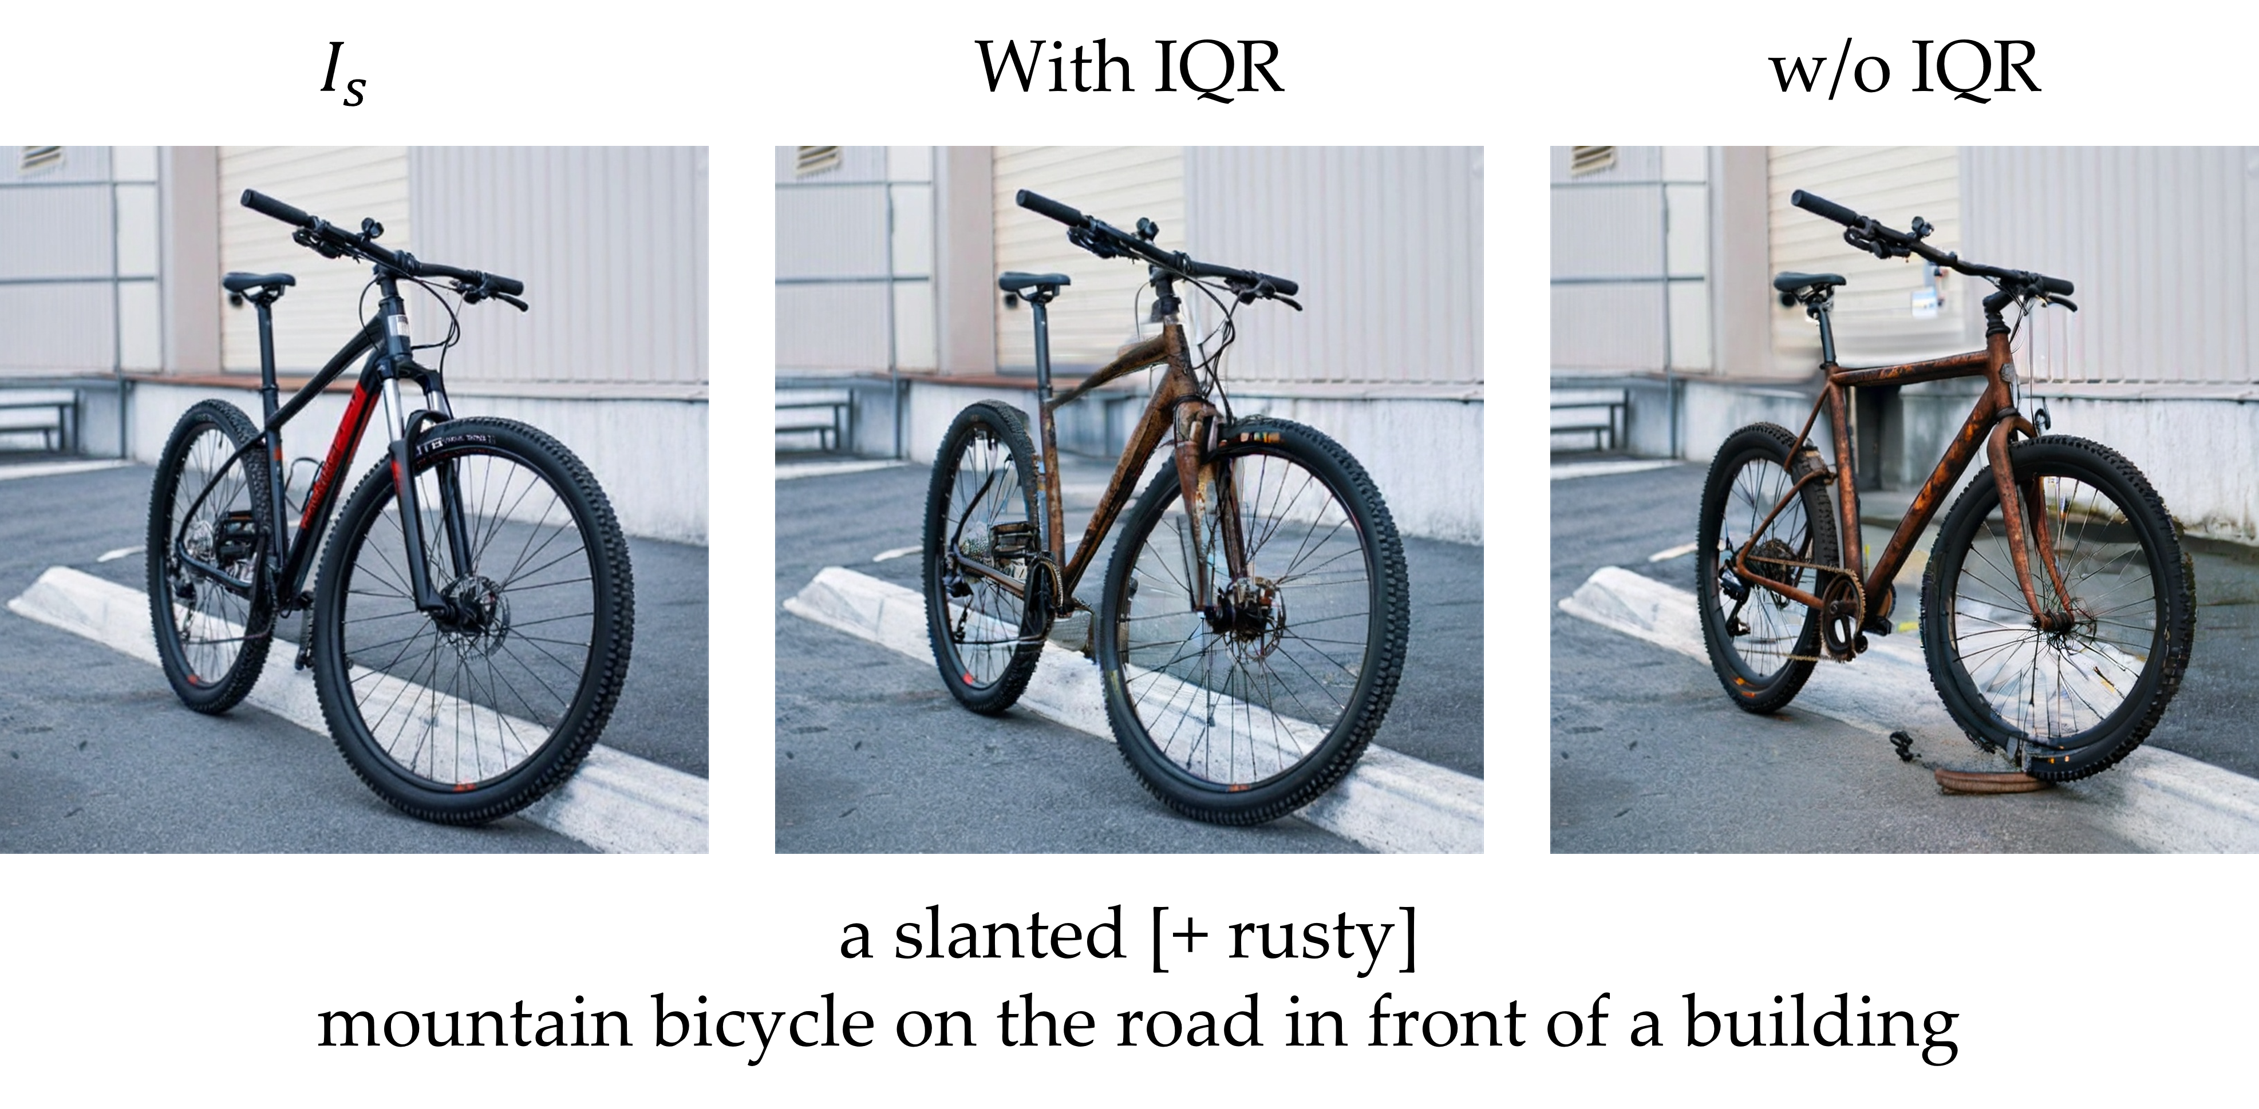
\includegraphics[width=\linewidth]{imgs/ablationIQR.png}
    \caption{Effect of IQR filtering. With filtering, the mask accurately captures the editing region and preserves the bicycle structure. Without it, the structure is severely distorted.}
    \label{fig:ablationIQR}
\end{figure}

As shown in Table~\ref{tab:ablation_iqr}, IQR filtering yields substantial improvements: PSNR increases by 14.0\% and SSIM by 8.8\%, while LPIPS drops by 35.2\%, confirming that filtered masks avoid corrupting non-target regions. Structure Distance also improves ($0.0328 \to 0.0316$), showing that cleaner masks reduce unintended structural changes. Fig.~\ref{fig:ablationIQR} illustrates the effect: without filtering, noisy attention from uninformative blocks produces imprecise masks that distort the bicycle structure; with IQR filtering, the mask cleanly delineates the target.
   % VI.   Experiments
\section{Discussion and Limitations}
\label{sec:limitations}

\subsection{Coarse-Scale Anchoring Bounds the Class of Feasible Edits}

The clearest limitation of the framework is inherited from the property that
makes it work. VAR commits to the global spatial arrangement within its first few
scales, and Sec.~\ref{sec:anchoring} shows that anchoring those scales to the
source is what keeps the background stable; the same anchoring necessarily
prevents an edit from rearranging the layout. The framework is therefore
well-suited to edits that keep the global composition --- replacement,
insertion, removal, attribute and style changes, and moderate pose adjustment ---
and unsuited to edits that demand a fundamentally different arrangement, such as
completely reorienting a subject's body (Fig.~\ref{fig:failure_cases}).

We emphasize that this is a measured trade-off with an exposed control rather
than a fixed rule. $N$ can be reduced, and Table~\ref{tab:ablation_mask} together
with Fig.~\ref{fig:shape_diff} quantifies what is bought and lost at each
setting: at small $N$ the layout is free but the background degrades, at large
$N$ the background is preserved and the subject is locked. Removing the anchoring
entirely is strictly worse than keeping it (Table~\ref{tab:anchoring}(a)). What
the present formulation cannot do is make that choice per region --- freeing the
layout where the edit needs it while anchoring it elsewhere --- because the
coarse scales carry too few tokens for a spatial mask to be meaningful. A
resolution-aware anchoring schedule, or an anchor that operates on the continuous
residual rather than on discrete tokens, is the natural next step.

\subsection{Composition Is Hard by Construction}

Composition substitutes tokens under a binary mask, which guarantees that
unedited regions decode exactly to the source but also prevents any interaction
--- lighting, shadow, contact --- across the mask boundary. In a preliminary
study we replaced the discrete substitution with a blend performed on the
continuous residual at full resolution, applying a single mask to the
interpolated codes of every scale before accumulation
(Fig.~\ref{fig:blend}). On the full benchmark this
raises PSNR from $22.8$ to $29.2$\,dB and halves both LPIPS and Structure
Distance, and it makes the target-stream pass unnecessary, reducing the pipeline
to two phases. It also costs roughly half the ImgReward, and three categories ---
object replacement, color change and background replacement --- are clearly worse,
since blending towards the source directly opposes what those edits require. We
report this as a characterization of the design space rather than as a
replacement for the method: hard composition and continuous blending occupy
different ends of a preservation-versus-edit-strength axis, and neither dominates.
\begin{figure}[t]
    \centering
    \begin{minipage}{0.245\linewidth}\centering
        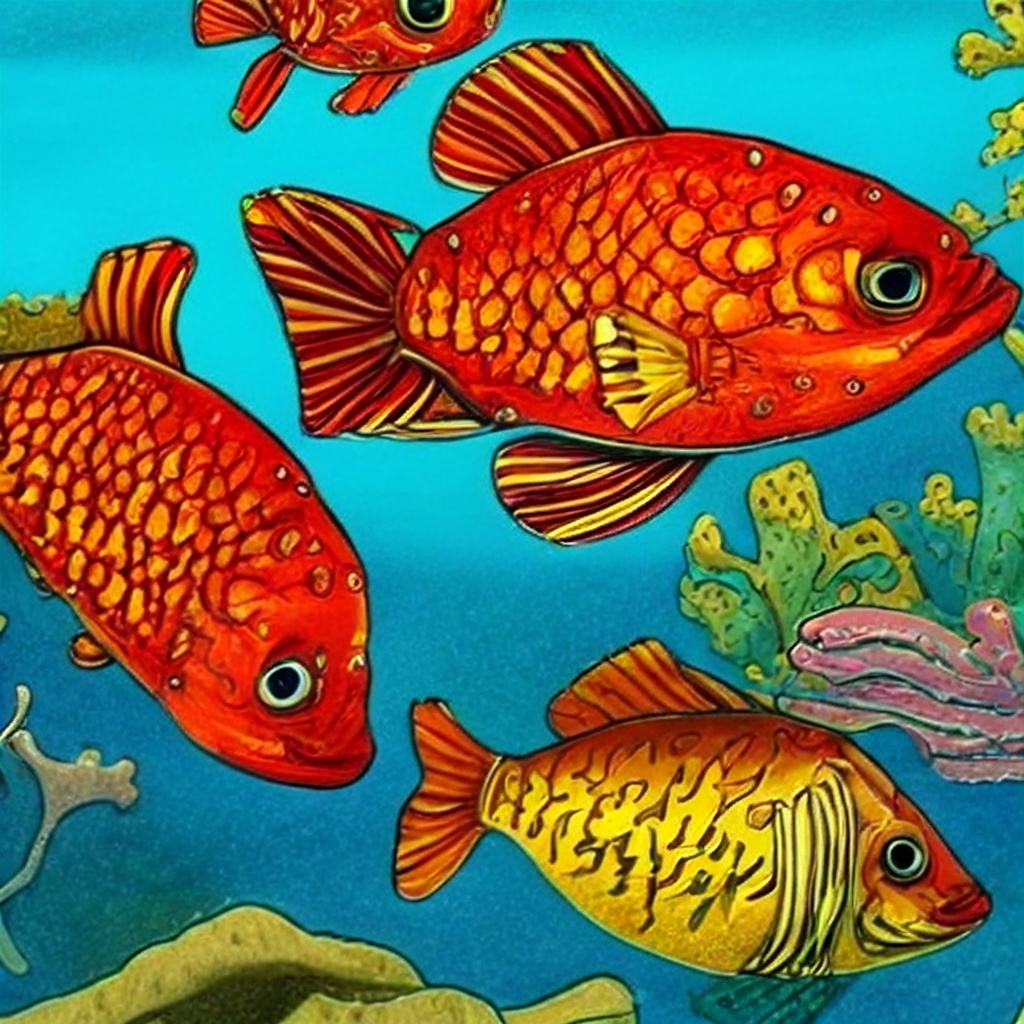
\includegraphics[width=\linewidth]{imgs/blend_source.jpg}\\{\footnotesize source}
    \end{minipage}\hfill
    \begin{minipage}{0.245\linewidth}\centering
        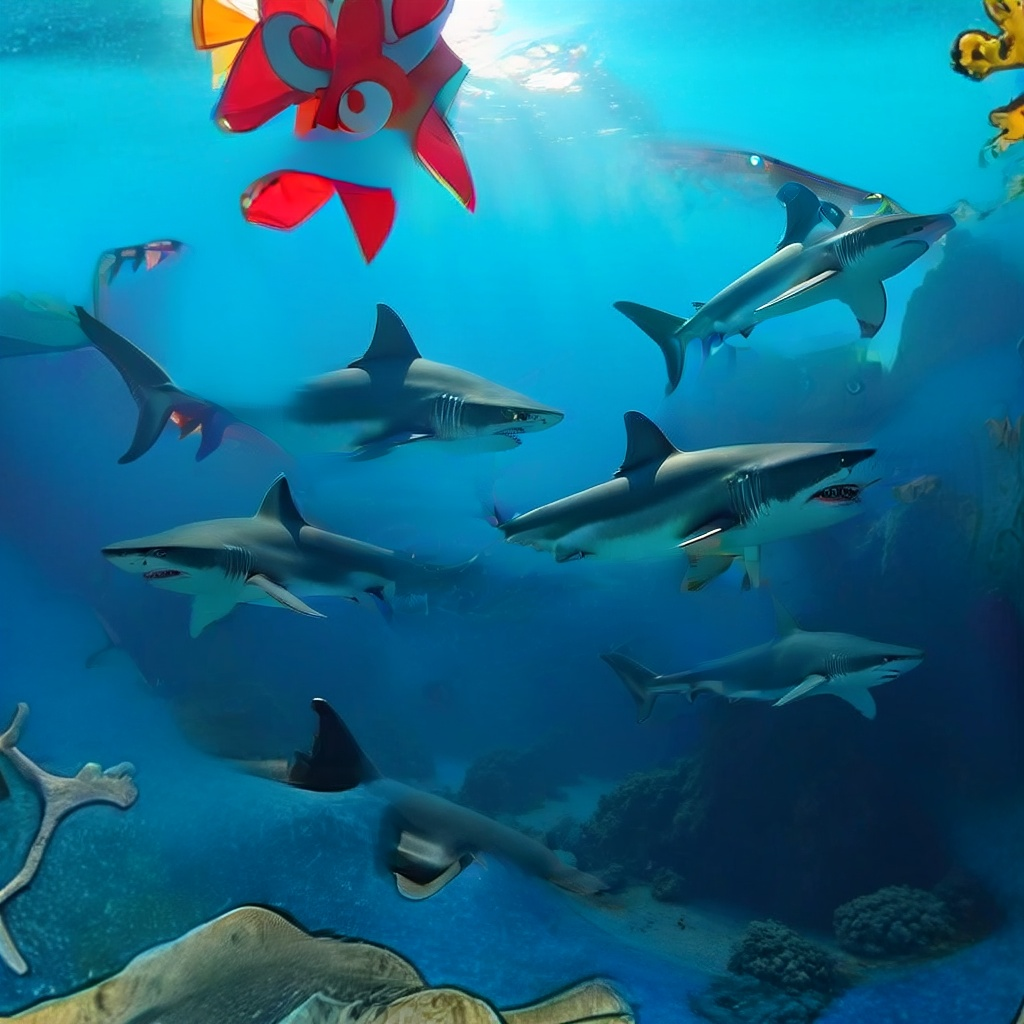
\includegraphics[width=\linewidth]{imgs/blend_baseline.jpg}\\{\footnotesize hard composition}
    \end{minipage}\hfill
    \begin{minipage}{0.245\linewidth}\centering
        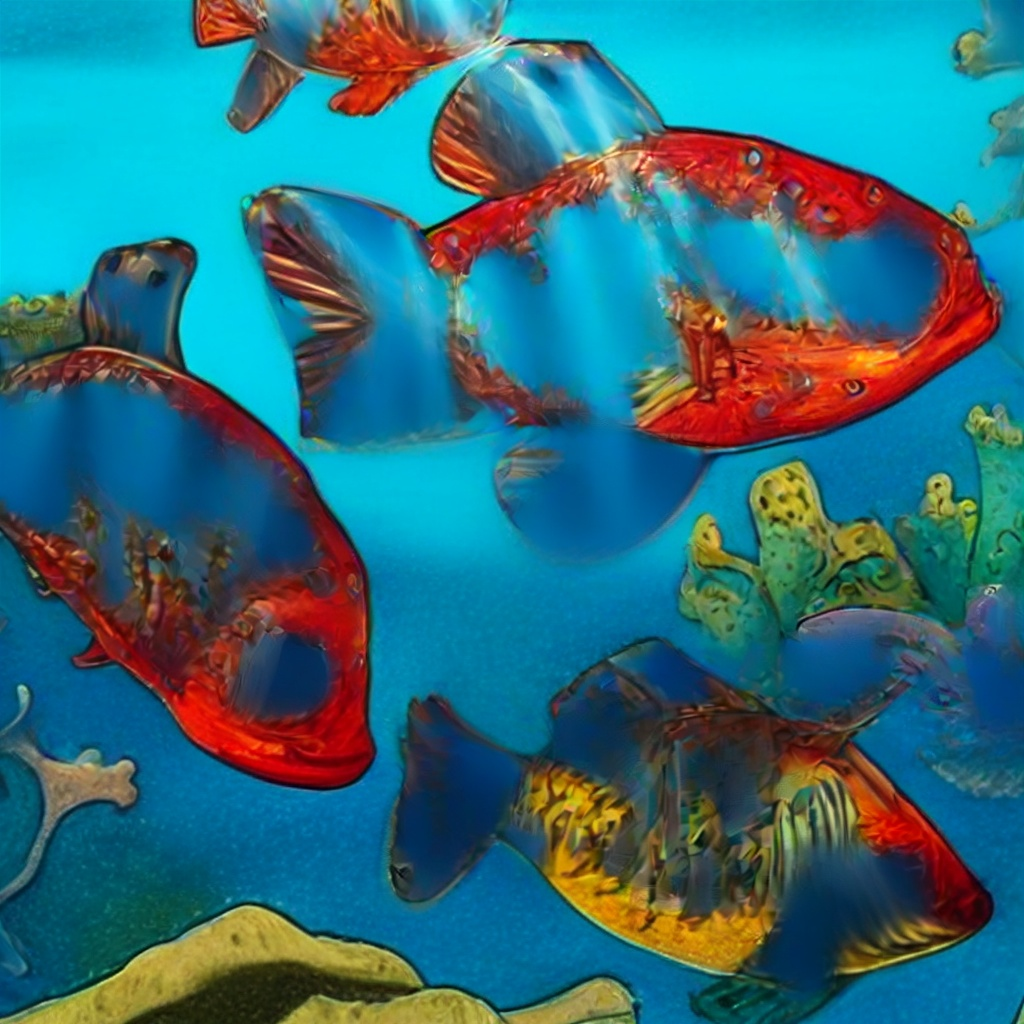
\includegraphics[width=\linewidth]{imgs/blend_hard.jpg}\\{\footnotesize blend, raw mask}
    \end{minipage}\hfill
    \begin{minipage}{0.245\linewidth}\centering
        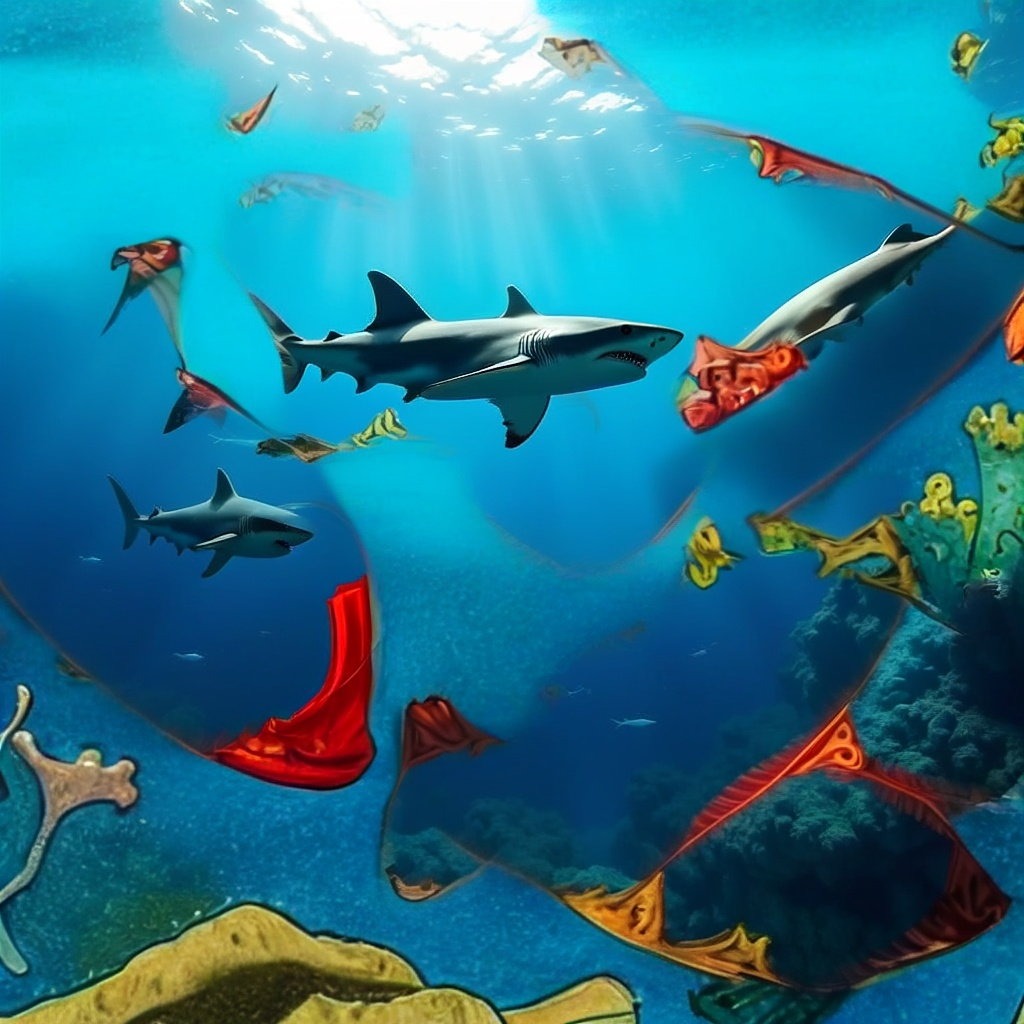
\includegraphics[width=\linewidth]{imgs/blend_best.jpg}\\{\footnotesize blend, cleaned mask}
    \end{minipage}
    \caption{Hard composition versus continuous blending (fish $\to$ shark). Hard composition executes the edit but drifts in style and loses much of the coral background. Blending the continuous residual at full resolution preserves both, but the last-scale attention mask is high-frequency and fragmented, so applying it directly leaves fragments of the source inside the edited region (third panel); a morphological closing and opening of the mask, a soft transition band and coarse anchoring recover the edit (fourth panel). Neither end of this axis dominates: see Sec.~\ref{sec:limitations}.}
    \label{fig:blend}
\end{figure}


% TODO(optional): promote this to a full subsection with its own table if the
% full-res blend results are included; source
% docs/new_exp/2026-07-22-fullres-blend-and-inverse-attention.md §2.

\subsection{The Threshold Is Global, Not Per Case}

A single $(h, c_{\max}, \kappa_{\max})$ is shared by every case, so the adaptation is driven only by the statistics of the attention map and not by how difficult the particular edit is. Choosing the operating point per case would require a signal that is not available before generation starts; predicting the whole metric-versus-threshold curve, or reading a signal after generation has begun, are the two natural routes and both are outside the scope of this paper.

\subsection{Dependence on Focus-Word Extraction}

Focus words are obtained by differencing the source and target prompts, which
assumes the two are structurally comparable. This assumption fails in two ways.
When the source prompt contains no anchor for the region to be edited --- most
commonly for object addition and style transfer, where the source description
simply does not mention the relevant region --- the source-side focus set is
empty and the pipeline falls back to a single-stream path. When the two prompts
are written independently and differ in phrasing rather than in content, the
difference contains words that are not edit-relevant. We quantify both cases in
Appendix~\ref{app:prompt}: on this benchmark, $230$ of $700$ source prompts yield
an empty focus set. A prompt encoder that identifies edit-relevant spans directly,
rather than by set difference, would remove the assumption entirely.
% TODO: write Appendix app:prompt from docs/reports/m14_minimal_rewrite_pipeline
% (experiments 4-5) and docs/reports/prompt_length_comparison_m15.  Keep the main
% tables free of the rewriting module: report it as an analysis of the failure
% mode plus an optional preprocessing step, not as part of the method.

\subsection{Backbone Dependence and Outlook}

Editing quality on fine textures is bounded by the reconstruction fidelity of the
backbone, and any bias of the base model propagates into the edit. The
mechanism itself, however, makes no assumption beyond next-scale prediction over
spatially localized discrete tokens with cross-modal attention. Recent extensions
of visual autoregressive modeling to video generate frames under the same
coarse-to-fine schedule, and the mask construction described here is orthogonal
to the temporal axis: the same per-scale focus and preserve masks can be built
from each frame's cross-attention and composed with the same token substitution
rule. Combined with an inference cost of about $2.5$\,s per image on a single
consumer GPU --- one to two orders of magnitude below inversion-based editors ---
this makes training-free editing of autoregressively generated video a concrete
next target rather than a speculative one.
    % VII.  Discussion and Limitations
\section{Conclusion}
\label{section:conclusion}

We presented a training-free, inversion-free image editing framework that brings
attention-driven spatial control to Visual Autoregressive Models. Cross-attention
maps inside a VAR transformer already carry enough spatial semantics to build
precise editing masks, provided that blocks dominated by positional bias are
removed and that the maps are binarized by an absolute energy level rather than
by rank; combined with the self-consistency of BSQ tokenization, this yields
background preservation by construction instead of by approximation.

Beyond the method itself, our analysis isolates what actually governs the
preservation--edit trade-off in this setting. The base threshold level traces a
smooth, monotone frontier and is the single control worth exposing; the
CV-adaptive correction shifts that frontier outward by an amount we quantify
against the fixed-threshold interpolation under two independent preservation
metrics; the target-stream pass contributes structurally rather than
parametrically, moving the entire frontier rather than the operating point along
it; explicit coarse anchoring dominates the implicit cumulative alternative; and
the preserve level, despite appearing as a hyperparameter, provably cannot affect
the output.

We believe the discrete, scale-wise structure of autoregressive generation is a
promising and still underexplored foundation for training-free image
manipulation, and that the mask construction demonstrated here transfers directly
to autoregressive video generation, where the same coarse-to-fine schedule
applies frame by frame.

\begin{figure}[t]
    \centering
    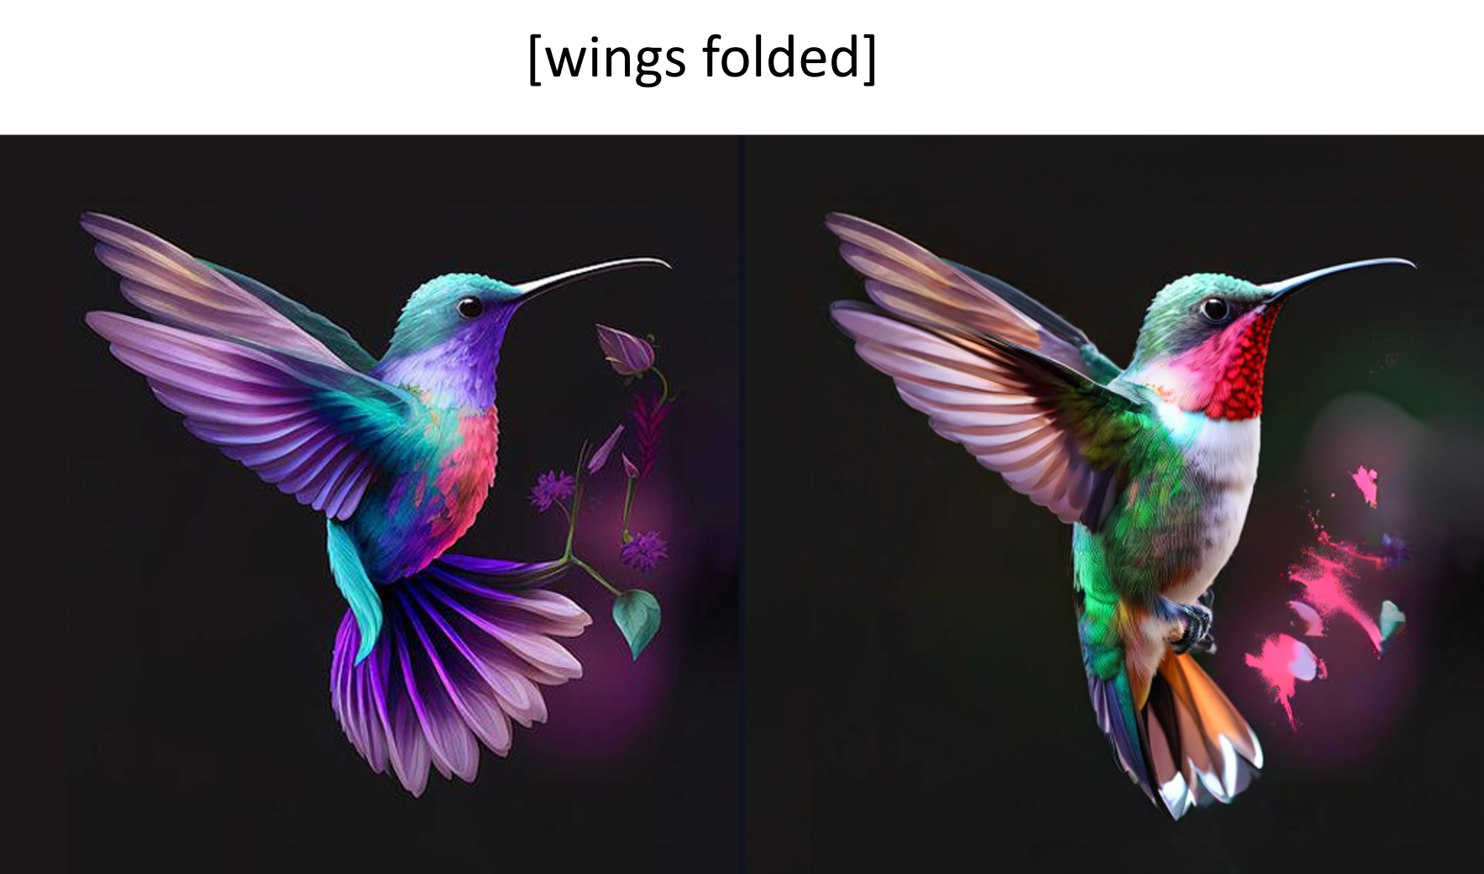
\includegraphics[width=0.75\linewidth]{imgs/failure_cases.png}
    \caption{Failure case: drastic pose changes conflict with coarse-scale structural anchoring.}
    \label{fig:failure_cases}
\end{figure}
    % VIII. Conclusion

% ---------------------------------------------------------------------------
\bibliographystyle{IEEEtran}
\bibliography{main}

% ---------------------------------------------------------------------------
% Appendix.  TCSVT allows appendices in the main body; several sections that
% were supplementary-only in the ACM version now belong here.
\appendices
%% ===========================================================================
%%  APPENDICES.  Loaded after \appendices in main.tex.
%%
%%  Content that used to live here and has been PROMOTED to the main body:
%%    - Adaptive mask thresholding + Algorithm 1  -> Sec. IV-C
%%    - Complete editing pipeline, Algorithm 2    -> Sec. IV-D
%%    - Scale-level replacement analysis (Fig.)   -> Sec. VI-C
%% ===========================================================================

\section{Implementation Details}
\label{app:impl}

This appendix records the details needed to reproduce the pipeline exactly.

\noindent\textbf{Three generation passes, one set of weights.}
A single edit invokes the VAR transformer three times with identical weights and
seed. The passes differ only in four switches: whether continuous source features
are injected, which token storage is attached, whether the storage masks are
applied, and whether generated tokens are saved. Phase~1 injects the continuous
features at every scale with weight $0$, which replaces the accumulated residual
by the source features and makes the pass a reconstruction of $I_s$; Phase~2
attaches a storage holding the source bitwise tokens together with the preserve
mask, so background positions are pinned while the rest generates freely;
Phase~3 attaches the same tokens with the replacement mask.

\noindent\textbf{Which tokens are written back.}
The tokens substituted in Phase~3 are always the BSQ quantization of the source
image, obtained once before generation begins. The tokens produced by Phase~1 are
overwritten before Phase~3, and the tokens produced by Phase~2 are discarded.
Phase~2 therefore influences the output through exactly one channel, the target
focus mask --- which is the reason the preserve level $\ell$ is inert and the
reason removing Phase~2 altogether has a large effect
(Sec.~\ref{sec:ablation_phase2}).

\noindent\textbf{Mask polarity and granularity.}
Storage masks are \emph{replacement} masks, not protection masks: a true entry
means the position is copied from the source. Substitution operates on the
bitwise index $r_k \in \{0,1\}^{h_k \times w_k \times d}$ with $d{=}32$, so
composition is exact at the bit level and boundaries between replaced and
generated regions are resolved per bit.

\noindent\textbf{Attention extraction.}
Cross-attention is recorded by patching the forward pass of blocks $2$--$31$ and
recomputing $\mathrm{softmax}(qk^{\top}/\sqrt{d_h})$ from the module's own
weights, leaving the original output path untouched. Because VAR evaluates each
block exactly once per scale, the invocation counter of each block gives the
scale index directly. For a focus word spanning several text tokens, the
per-token maps are averaged; head dimensions are averaged before block-level
aggregation.

% TODO(optional): a data-flow figure of the three phases (mermaid source in
% docs/reports/p2p_three_phase_pipeline/report.md §0) would make this appendix
% considerably easier to follow.

\section{Evaluation Protocol}
\label{app:eval}

\noindent\textbf{Metrics.}
Structure Distance, and PSNR / SSIM / LPIPS / MSE restricted to the unedited
region, follow the official PIE-Bench implementation. CLIP whole and CLIP edited
use the standard CLIP score on the full image and on the annotated edited region
respectively. We additionally report HPSv2 (version 2.1) and ImageReward.

\noindent\textbf{Prompt convention.}
All preference and CLIP scores are computed against the \emph{original}
PIE-Bench editing prompt, with bracket annotations removed, regardless of which
prompt was used for generation. This matters: scoring a generation against a
paraphrased prompt instead of the original changes ImageReward by up to $0.33$
and HPSv2 by $0.025$ on this benchmark, which is larger than most of the effects
studied in Sec.~\ref{sec:analysis}. Any comparison that mixes the two conventions
is meaningless.

\noindent\textbf{Resolution handling.}
Edited images are resized to the source resolution with Lanczos resampling before
any metric is computed.

\noindent\textbf{Run-to-run noise.}
Generation uses bf16 kernels with fused attention and is not bit-exact. Repeating
a full-benchmark run under an identical configuration and seed changes the mean
by $\approx\!\pm 0.02$ ImageReward and $\approx\!\pm 0.001$ HPSv2 at $n{=}700$,
and by $\approx\!\pm 0.05$ ImageReward for an individual $n{=}80$ category. We
state this scale wherever a reported difference approaches it.

\section{Text-to-Image Editing Mode}
\label{app:t2i}

% TODO: move the T2I qualitative results here from the ACM supplementary
% material, and describe the mask-mechanism validation performed in this mode.

\section{Focus-Word Extraction: Failure Modes}
\label{app:prompt}

% TODO: write from docs/reports/m14_minimal_rewrite_pipeline (experiments 4-5)
% and docs/reports/prompt_length_comparison_m15.  Points to cover:
%   - 230/700 source prompts yield an empty focus set; concentrated in
%     add_object (75/80) and change_style (76/80).
%   - A conditional minimal patch (insert an anchor into the source prompt only,
%     leave the target prompt untouched) recovers +0.19 to +0.41 ImageReward on
%     the patched categories at no preservation cost.
%   - Rewriting whole prompts is strictly harmful and monotone in length
%     (IR 0.653 -> 0.372 -> 0.206 for original / short rewrite / long rewrite),
%     because generation follows the rewritten prompt while scoring uses the
%     original one.  This is the prompt-convention effect quantified in
%     Appendix~\ref{app:eval}, not a property of the editing method.
%   - Keep the main tables free of the rewriting module.

\section{Additional Qualitative Results}
\label{app:qualitative}

% TODO: 2-3 examples per editing category.  A journal appendix has the space and
% this is the cheapest way to answer "evaluation scope is narrow".


% ---------------------------------------------------------------------------
% Author biographies (TCSVT requires them for the final version).
% \begin{IEEEbiography}[{\includegraphics[width=1in,height=1.25in,clip,keepaspectratio]{photo}}]{Author Name}
% Biography text here.
% \end{IEEEbiography}

\end{document}
